%%%%%%%%%%%%%%%%%%%%%
% Documento maestro %
%%%%%%%%%%%%%%%%%%%%%
\documentclass[oneside]{fime}


%%%%%%%%%%%%%%%%%%%%%%%%%%%%%%%%%%%%%%%%%%%
% Cargando paquetes y definiendo opciones %
%%%%%%%%%%%%%%%%%%%%%%%%%%%%%%%%%%%%%%%%%%%
% Aquí puedes cargar los paquetes que vas a usar. La clase
% fime ya incluye babel, inputenc, graphicx y los de la AMS.
% Cargar un paquete está a tu libertad (y responsabilidad).

\usepackage{hyperref}
	\hypersetup{breaklinks=true,colorlinks=true,linkcolor=black,citecolor=black,urlcolor=black}
\usepackage[toc, section=chapter, nopostdot]{glossaries}
	\makenoidxglossaries	
	\loadglsentries{Glosario}
	\setglossarystyle{altlist}
\usepackage{subfig}
\usepackage[numbers, sort&compress]{natbib}
\usepackage{adjustbox}
\usepackage{amssymb}% http://ctan.org/pkg/amssymb
\usepackage{pifont}% http://ctan.org/pkg/pifont
	\newcommand{\cmark}{\ding{51}}%
	\newcommand{\xmark}{\ding{53}}%


%%%%%%%%%%%%%%%%%%%%%
% Definiendo campos %
%%%%%%%%%%%%%%%%%%%%%
\def\titulo{Detección de melanoma de piel mediante segmentación semántica}
\def\autor{Mario Alberto Flores Hernández}
\def\matricula{1719126}
\def\grado{Licenciatura en Ingeniería en Mecatrónica}
% En caso de que el grado tenga orientación o especialidad llenar el siguiente
% campo dejando un ESPACIO INICIAL, en caso contrario, dejar vacío
\def\orientacion{}
% Coloca el mes con mayúscula inicial
\def\fecha{Febrero 2021}

\def\asesor{Dra. Satu Elisa Schaeffer}
\def\revisorA{Dr. Romeo Sánchez Nigenda}
\def\revisorB{Dra. Sara Elena Garza Villarreal}
% En el caso de que tu tesis sea de doctorado activa la variable cambiándola a \doctoradotrue
% y define tus otros dos revisores
\newif\ifdoctorado\doctoradofalse
% El visto bueno siempre va
\def\vobo{Dr. Fernando Banda Muñoz}




%%%%%%%%%%%%%%%%%%%%%%%
% Inicia el documento %
%%%%%%%%%%%%%%%%%%%%%%%
\begin{document}

\frontmatter
\pagestyle{main}

%%%%%%%%%%%%%%%%%%%%%%%%
% Primer portada: UANL %
%%%%%%%%%%%%%%%%%%%%%%%%
\thispagestyle{empty}

\begin{scshape}
\begin{center}
	{\Large \uanl} \\[5mm]
	{\large \fime} \\[5mm]
	{\large \depg}
	\vskip15mm
	
\includegraphics[height=55mm]{uanl}
	\vskip12mm
	\begin{tabular}{p{11cm}}
		\centering
		{\large \titulo}
	\end{tabular}
	\vskip7mm
	{por}\\[7mm]
	{\large \autor}\\[7mm]
        % Si en tu posgrado la tesis no es opcional (como sí lo es en licenciatura), no modifiques esta línea:
	{como requisito parcial para obtener el grado de}\\[3mm]
	\MakeUppercase{\grado}\\
	\orientacion
	\vfill
	\fecha
\end{center}
\end{scshape}

%%%%%%%%%%%%%%%%%%%%%%%%%
% Segunda portada: FIME %
%%%%%%%%%%%%%%%%%%%%%%%%%
\newpage
\thispagestyle{empty}

\begin{scshape}
\begin{center}
	{\Large\uanl} \\[5mm]
	{\large\fime} \\[5mm]
	{\large\depg}
	\vskip16mm
	
\includegraphics[height=50mm]{fime}
	\vskip16mm
	\begin{tabular}{p{11cm}}
		\centering
		{\large \titulo}
	\end{tabular}
	\vskip7mm
	{por}\\[7mm]
	{\large \autor}\\[7mm]
        % Si en tu posgrado la tesis no es opcional (como sí lo es en licenciatura), no modifiques esta línea:
	{como requisito parcial para obtener el grado de}\\[3mm]
	\MakeUppercase{\grado}\\
	\orientacion
	\vfill
	\fecha
\end{center}
\end{scshape}

%%%%%%%%%%%%%%%%%%%%%%%%%%%%%
% Carta del comité de tesis %
%%%%%%%%%%%%%%%%%%%%%%%%%%%%%
\newpage
\thispagestyle{empty}
\enlargethispage{5mm}

{\renewcommand{\baselinestretch}{1.1}\selectfont
\begin{center}\vspace*{-25mm}\hspace*{-10mm}
\begin{minipage}{170.5mm}
\hspace{-1.5mm}
\includegraphics[height=20mm]{uanl}\hfill\raise1mm\hbox{
\includegraphics[height=18.5mm]{fime}}
\hrule\vspace{0.5mm}
\scalebox{.5}{\MakeUppercase{\uanl}}\hfill\scalebox{.5}{\MakeUppercase{\fime}}\medskip
\end{minipage}
\vskip4mm{\sc\large\uanl\\\fime\\[3pt]\depg}\vskip6mm
\end{center}

Los miembros del Comité de Tesis recomendamos que la Tesis <<\titulo>>, realizada por el alumno \autor, con número de matrícula \matricula, sea aceptada para su defensa como requisito parcial para obtener el grado de \grado\orientacion.
\ifdoctorado\vskip10mm\else\vskip8mm\fi

\begin{center}
El Comité de Tesis\\
\ifdoctorado\vskip15mm\else\vskip25mm\fi

\ifdoctorado{%%%
\begin{tabular}{p{37mm}p{21mm}p{12mm}p{21mm}p{37mm}}
	\cline{2-4}
	& \multicolumn{3}{c}{\asesor} & \\
	& \multicolumn{3}{c}{Asesor}  & \\[15mm]
	\cline{1-2} \cline{4-5}
	\multicolumn{2}{c}{\revisorA} & & \multicolumn{2}{c}{\revisorB} \\
	\multicolumn{2}{c}{Revisor}   & & \multicolumn{2}{c}{Revisor}   \\[17mm]
	\cline{1-2} \cline{4-5}
	\multicolumn{2}{c}{\revisorC} & & \multicolumn{2}{c}{\revisorD} \\
	\multicolumn{2}{c}{Revisor}   & & \multicolumn{2}{c}{Revisor}   \\[2mm]
	& \multicolumn{3}{c}{Vo. Bo.} & \\[14mm]
	\cline{2-4}
	& \multicolumn{3}{c}{\vobo}   & \\
	& \multicolumn{3}{c}{Subdirector de Estudios de Posgrado}   & \\ &&&&
\end{tabular}
}\else{%%%
\begin{tabular}{p{37mm}p{21mm}p{12mm}p{21mm}p{37mm}}
	\cline{2-4}
	& \multicolumn{3}{c}{\asesor} & \\
	& \multicolumn{3}{c}{Asesora}  & \\[19mm]
	\cline{1-2} \cline{4-5}
	\multicolumn{2}{c}{\revisorA} & & \multicolumn{2}{c}{\revisorB} \\
	\multicolumn{2}{c}{Revisor}   & & \multicolumn{2}{c}{Revisora}   \\[2mm]
	& \multicolumn{3}{c}{Vo. Bo.} & \\[17mm]
	\cline{2-4}
	& \multicolumn{3}{c}{\vobo}   & \\
	& \multicolumn{3}{c}{Subdirector Académico}   & \\ &&&&
\end{tabular}
}\fi%%%

\vfill

\snnl, \MakeLowercase{\fecha}

\end{center}}

\tableofcontents

\listoffigures
\addcontentsline{toc}{chapter}{Índice de Figuras}

\listoftables
\addcontentsline{toc}{chapter}{Índice de Cuadros}

\chapter{Notaciones}

A continuación se resumen las notaciones usadas a lo largo de este trabajo de tesis, incluyendo el símbolo,  significado y equivalente en el idioma inglés.

\begin{itemize}
    \item $x$, dato de entrada (input).
    \item $y$, dato de salida (output).
    \item $\hat{y}$, salida estimada (estimated output).
    \item $d$, dimensión de entrada (input dimension).
    \item $d_{\rm o}$, dimensión de salida (output dimension).
    \item $n_s$, número de muestras (samples).
    \item $e_i$, entrada del nodo (node input).
    \item $p_i$, peso entre la entrada y el nodo (weight).
    \item $\phi$, función de activación (activation).
\end{itemize}


%Agradecimientos

\chapter{Agradecimientos}
\markboth{Agradecimientos}{}
\coltext{
Aquí puedes poner tus agradecimientos. (No olvides agradecer a tu comité de tesis, a tus profesores, a la facultad y a CONACyT en caso de que hayas sido beneficiado con una beca).
}

%Resumen

\chapter{Resumen}
\markboth{Resumen}{}

{\renewcommand{\baselinestretch}{1.1}\selectfont
{\setlength{\leftskip}{10mm}
\setlength{\parindent}{-10mm}

\autor.

Candidato para obtener el grado de \grado\orientacion.

\uanl.

\fime.

Título del estudio: \textsc{\titulo}.

\noindent Número de páginas: \pageref*{lastpage}.}

%%% Comienza a llenar aquí
\paragraph{Objetivos y método de estudio:}
Desarrollar una herramienta de asistencia para la detección de cáncer de piel utilizando las técnicas mas actuales de visión computacional e inteligencia artificial, se pretende desarrollar mediante \emph{software} y tecnicas de \emph{\gls{seg}} una aplicación que permita introducir una imagen y como resultado obtengamos un mapa de características segmentado en una o más categorías. 

\paragraph{Contribuciones y conclusiones:}
\coltext{}
\newline

\bigskip\noindent\begin{tabular}{lc}
\vspace*{-2mm}\hspace*{-2mm}Firma del asesor: & \\
\cline{2-2} & \hspace*{1em}\asesor\hspace*{1em}
\end{tabular}}



\mainmatter
\pagestyle{fime}


%%% Haz un documento para cada capítulo


\chapter{Introducción}

La piel es considerada como el órgano más grande del cuerpo humano; está compuesta por tres capas: \emph{\gls{epidermis}}, \emph{\gls{dermis}} e \emph{\gls{hipodermis}}, tal como se ilustra en la figura \ref{fig:skin1_jpg}. La función principal de la piel es la de proteger al cuerpo de las hostilidades del medio ambiente tales como la radiación solar y los factores externos como las bacterias, proteger a los órganos y otros tejidos internos, y también funciona como una interfaz que nos permite interactuar con el medio ambiente otorgándonos la capacidad de percibir sensaciones tales como el tacto y la temperatura.

\begin{figure}[h!]
    \includegraphics[scale = 1.0]{Figuras/skin_structure_esp.eps}
    \centering
    \caption{Ilustración de las capas de la piel y sus apéndices \citep{skin_1}.}
    \label{fig:skin1_jpg}
\end{figure}

Sin embargo, debido a la exposición continua a la radiación solar o artificial, un porcentaje de la población llega a desarrollar anomalías relacionadas a la piel. Una de estas anomalías es la denominada \emph{melanoma}, la cuál es una mutación originada en los melanocitos (células encargadas de otorgar la pigmentación marrón a la piel), en donde estas células crecen sin control y se esparcen a otras partes del cuerpo, ocasionando graves daños a la salud de quien la padece y que sin una detección temprana puede aumentar rápidamente el riesgo de fallecimiento \citep{cancer_org}.

\begin{figure}[h!]
    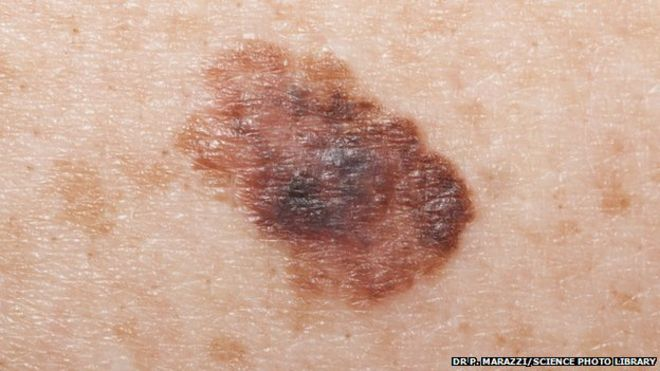
\includegraphics[width=80mm]{Figuras/skin_cancer_bbc.jpg}
    \centering
    \caption{Ejemplo de melanoma \citep{cancer_img_1}.}
    \label{fig:can_jpg}
\end{figure}

 Su detección temprana es imprescindible para reducir el porcentaje de mortalidad que esta enfermedad representa, de ahí el porqué es importante no solamente trabajar en encontrar un tratamiento, sino también (y de forma simultánea), trabajar e investigar en el uso de tecnologías emergentes que permitan su detección temprana, confiable y al alcance de la mayoría.

En los últimos años se han logrado muchos avances en cuanto al desarrollo de \emph{software} inteligente, una de las tecnologías que han adquirido mayor importancia es la \emph{\gls{rn}}, la cual se trata de un modelo matemático que tiene la capacidad de \emph{aprender} mediante el uso de bases de datos y mediante funciones de optimización que permite la configuración de dicho modelo y le otorga la capacidad de predecir, clasificar o construir datos ya sean futuros o desconocidos. Algunos de los sectores que se han beneficiado más de esta tecnología son: el sector automotriz (pilotos automáticos), el sector de manufactura (optimización de procesos), el sector de entretenimiento (recomendaciones personalizadas), el sector médico (diagnóstico de imágenes). 


\section{Hipótesis}
El presente trabajo de tesis tiene como hipótesis el uso de la inteligencia artificial para la detección y clasificación del melanoma de piel; mediante la implementación de un modelo basado en el aprendizaje profundo, es posible crear una aplicación de \emph{software} que entrene y optimice un modelo para realizar la tarea de la \emph{segmentación semántica}, la cual se trata de la transformación y predicción de pixeles para obtener la clasificación de las diferentes regiones que representa una imágen dermatológica. Y de esta manera obtener una aplicación de reconocimiento visual cuya robustez pueda ser verificada a partir de una serie de experimentos.


%Es posible clasificar los píxeles en distintas categorías dentro de una %imagen gracias a las avances actuales de inteligencia artificial y la técnica %de segmentación. Mediante la técnica de \emph{\gls{seg}} es posible crear un %reconocedor visual que no solo detecte la presencia y ubicación del elemento %a reconocer, sino que, también obtenga otros datos descriptivos del elemento %como el tamaño, forma y región que abarca dentro de la imagen.

\section{Objetivos}
Primero en \emph{objetivo general}, se habla de manera conceptual la problemática a resolver tales como cuales son las situaciones en las que podemos optimizar la solución de un problema mediante el uso de la red neuronal, posteriormente en los \emph{objetivos específicos} se describe de forma puntual los pasos a realizar en el presente trabajo de tésis para llegar al resultado deseado.

El \emph{objetivo general} de este trabajo de tesis es la creación de una aplicación con la capacidad de reconocer y segmentar melanoma en la piel de forma automatizada, esto con el motivo de asistir a los médicos dedicados a esta labor a optimizar y extender la detección temprana, consiguiendo así reducir la tasa de mortalidad de este padicimiento.

El \emph{objetivo específico}, es el de implementar un modelo de red neuronal cuya entrada sean imágenes que pueden o no contener la presencia de alguno de los tipos de cáncer de piel comunes, y como salida del modelo se obtenga un mapa de características donde de haber presencia del cáncer, éste se distinga mediante una región colorada en el espacio que abarca. El modelo debe cumplir con las siguientes características:

\begin{itemize}
    \item El modelo debe ser capaz de trabajar con imágenes a color o en blanco y negro.
    \item El modelo debe contar con una función capaz de evaluar la precisión.
    \item El modelo debe contar con un algoritmo capaz de optimizar la precisión.
    \item El modelo debe ser capaz de segmentar correctamente en imágenes no utilizadas en los datos de entrenamiento.
\end{itemize}

\begin{figure}[!htp]
    \centering
    \subfloat[imágen entrante]{\label{a_1}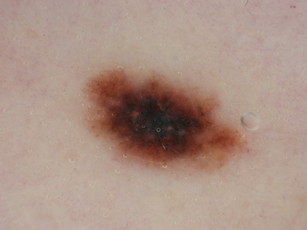
\includegraphics[width=50mm]{Figuras/input_1.png}}
    \qquad
    \subfloat[máscara de salida]{\label{b_1}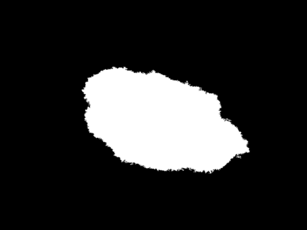
\includegraphics[width=50mm]{Figuras/mask_1.png}}
    \caption{Ejemplo de segmentación: entrada y salida.}
    \label{data_1}
\end{figure}

En la figura \ref{a_1} se observa como la imagen entrante presenta un caso de melanoma, mientras que la figura \ref{b_1} se puede observar la misma imagen después de pasar por una secuencia de transformaciones, esto se denomina \emph{segmentación semántica} y se refiere a la acción de separar y clasificar en una o más categorías los objetos detectables en una imagen.

\section{Estructura de la Tesis}
A continuación se da una breve explicación sobre el orden en el que se presentan los capítulos de este trabajo de tesis, así como una breve descripción de su contenido.

En el capítulo 2 se habla sobre los antecedentes relacionados al presente trabajo de tesis, primero se empieza definiendo la naturaleza del problema con el que se pretende tratar, después algúnos conceptos clave que serán necesarios para la comprensión de la implementación propuesta tales como las dimensiones de los datos y los algoritmos de evaluación y optimización.

En el capítulo 3 se recopilan trabajos relacionados al método o problemática en cuestión, se estudia las características de dichos trabajos y se busca un punto de convergencia entre estos y el presente trabajo de tésis con el fin de comparar las áreas de oportunidad.

En el capítulo 4 se define el proceso de transformación de los datos del sistema propuesto en este trabajo de tesis, desde las características de los datos a la entrada.

El capítulo 5 describe a profundidad la implementación de la propuesta, desde la descripción de los datos utilizados para el entrenamiento del modelo y la verificación de este, la arquitectura específica utilizada 


Finalmente, en el capítulo 6 se exponen los resultados obtenidos de la implementación del producto científico en el capítulo anterior, así como un análisis y conclusión final sobre los valores obtenidos en precision y tiempo de entrenamiento. 

\chapter{Antecedentes}
En este capítulo se introducen de forma teórica los conceptos relacionados con el trabajo propuesto, primero se define que es el \emph{cáncer de piel}, cuales son los factores que influyen en el desarollo de este padecimiento, los tipos de cáncer y las diferencias entre estos. Después algunos conceptos relacionados con las redes neuronales necesarios para un entendimiento sólido del \emph{aprendizaje profundo}, tales como los elementos clave que conforman a la red neuronal, la manera en la que esta evalúa su precisión, y el algoritmo de optimización.

\section{Cáncer de Piel}
El \emph{cáncer de piel} es una enfermedad que suele relacionarse con la aparición de lunares o manchas que no se encontraban previamente, se pueden manifestar como manchas oscuras o rojizas, bultos y/o escamas en la superficie de la piel y afecta a todos los tonos de piel por igual. Esta enfermedad se suele desarrollar principalmente en partes del cuerpo expuestas al sol, sin embargo, también se puede desarrollar en partes que no suelen exponerse. Algunos factores como la exposición a los rayos ultravioletas (rayos UV), el uso de sustancias como el tabaco o el envejecimiento son factores correlacionados con la aparición del \emph{cáncer de piel}, existen dos tipos de factores: \emph{intrínsecos} y \emph{extrínsecos}.

Los factores \emph{intrínsecos} son aquellos que suceden de forma interna en la piel, un ejemplo de esto es el envejecimiento cronológico, el cual es un proceso natural que consiste en degradación del colágeno, la elastina y el adelgazamiento de la epidermis debido al envejecimiento celular al paso de los años y de el efecto de algunas hormonas.
\bigskip

Los factores \emph{extrínsecos} son aquellos que suceden de forma agena al organismo, como es el caso del \emph{foto-envejecimiento} el cual sucede cuando nos encontramos expuestos a los rayos ultravioletas (UV). Este factor de envejecimiento genera lesiones en las cadenas de ácido desoxirribonucleico (ADN) debido a la oxidación y afecta la regeneración de celulas, al sistema inmune y a la forma en la que se regula la pigmentación \citep{skin_aging}.

\subsection{Tipos de Cáncer de Piel}
El cáncer de piel es un padecimiento que se puede manifestar en una gran variedad de formas distintas, algúnas de estas formas pueden representar un enorme riesgo para la salud de quien la padece mientras que otras pueden permanecer mucho tiempo sin afectar la calidad de vida del paciente; se clasifican principalmente en dos tipos: \emph{benigno} y \emph{maligno}.

Los tumores del tipo \emph{benignos} no suelen ser considerados cáncer como tal, ya que tienen un crecimiento lento y no suelen extenderse a otras partes del cuerpo, por otro lado los tumores \emph{malignos}, si representan un riesgo mayor ya que crecen rápidamente y suelen hacer \emph{metástasis}, lo cual significa que migra a otras partes del cuerpo.

\section{Redes Neuronales}

Hasta hace algunos años el desarrollo de aplicaciones de software solía realizarse de forma robústa, por ejemplo, si deseáramos desarrollar una aplicación de reconocimiento de imágenes faciales de la forma tradicional, sería necesario un grupo de expertos en dicho rubro para que definan una secuencia de transformaciones específicas para lograr esa función, donde la variabilidad de las imágenes que dicho sistema permitiría depende únicamente de la complejidad del mismo, sin embargo mediante las redes neuronales es posible resolver el mismo problema con la ventaja de que la variabilidad de imágenes que pueden ser reconocidas por el sistema, depende de los datos utilizados para el entrenamiento, el model de una red neuronal \emph{aprende} de los datos proporcionados y crea un modelo capaz de clasificar, predecir o reconstruir datos conocidos y desconocidos. Algunos de los puntos clave que conforman un sistema basado en redes neuronales son:

\begin{description}
    \item[Datos]{Se debe determinar la naturaleza y la dimensión de los datos que entrarán al modelo.}
    \item[Modelo] {Se debe crear un sistema que transforme los datos de entrada, en la salida deseada.}
    \item[Evaluación] {El modelo debe tener la capacidad de evaluar su precisión.}
    \item[Optimización] {El modelo debe contar con un algoritmo que optimice la precisión.}
\end{description}

\subsection{Imágenes como Datos}
Las imágenes se pueden definir como una matriz de $m \times n \times 1$ pixeles en el caso de las imágenes de un solo canal (blanco y negro) y en el caso de imágenes a color es de $m \times n \times k$, donde $k$ es igual al número de canales de color que tenga la imagen, siendo tres en el caso de imágenes RGB\footnote{RGB: Se refiere a los tres canales de color rojo, verde y azul, por sus siglas en inglés (\emph{red, green, blue}).}, es importante definir si las imágenes ingresarán al modelo a color o en blanco y negro debido a que esto define el número de nodos de entrada de este, ya que para cada pixel debe corresponder un nodo de entrada y en el caso de imágenes a color también deberá tener un número de capas de nodos de entrada igual al número de canales que tenga la imagen.

\definecolor{red_matrix}{rgb}{0.6, 0, 0}
\definecolor{green_matrix}{rgb}{0, 0.8, 0}
\definecolor{blue_matrix}{rgb}{0, 0.25, 1}

\begin{figure*}[htp]
    \centering
    \subfloat[Escala de grises.]{
        \label{mtr_1}
        
\begin{tikzpicture}
            \draw[step=5mm, black, line width=0.30mm] (-2,-2) grid (2,2);
        \end{tikzpicture}
    }
    \qquad
    \subfloat[A color.]{
        \label{mtr_2} 
        \begin{tikzpicture}
            \draw[step=5mm, red_matrix, line width=0.30mm] (-2.5,-2.5) grid (1.5,1.5);
            \draw[step=5mm, green_matrix, line width=0.30mm] (-2,-2) grid (2,2);
            \draw[step=5mm, blue, line width=0.30mm] (-1.5,-1.5) grid (2.5,2.5);
        \end{tikzpicture}
    }
    \caption{Comparación de las dimensiones entre los distintos canales de color.}
\end{figure*}

\subsection{Modelo}
Un \emph{modelo} se puede definir como el bloque intermedio entre los datos de entrada (\emph{input}) y los datos de salida (\emph{output}), es el sistema encargado de transformar los datos de entrada en la salida deseada y consta de los siguientes componentes:

La unidad principal que compone el modelo de la red neuronal es el perceptrón, denominado \emph{nodo} en esta literatura. Se trata de una analogía matemática basada en el comportamiento de la neurona biológica, el nodo recibe $n$ entradas, las cuales son multiplicadas por el peso $p$, se suma el producto de las entradas por sus pesos $ e \times p$ y finalmente se multiplica por la función de activación $\phi$. 

\begin{figure}[b]
    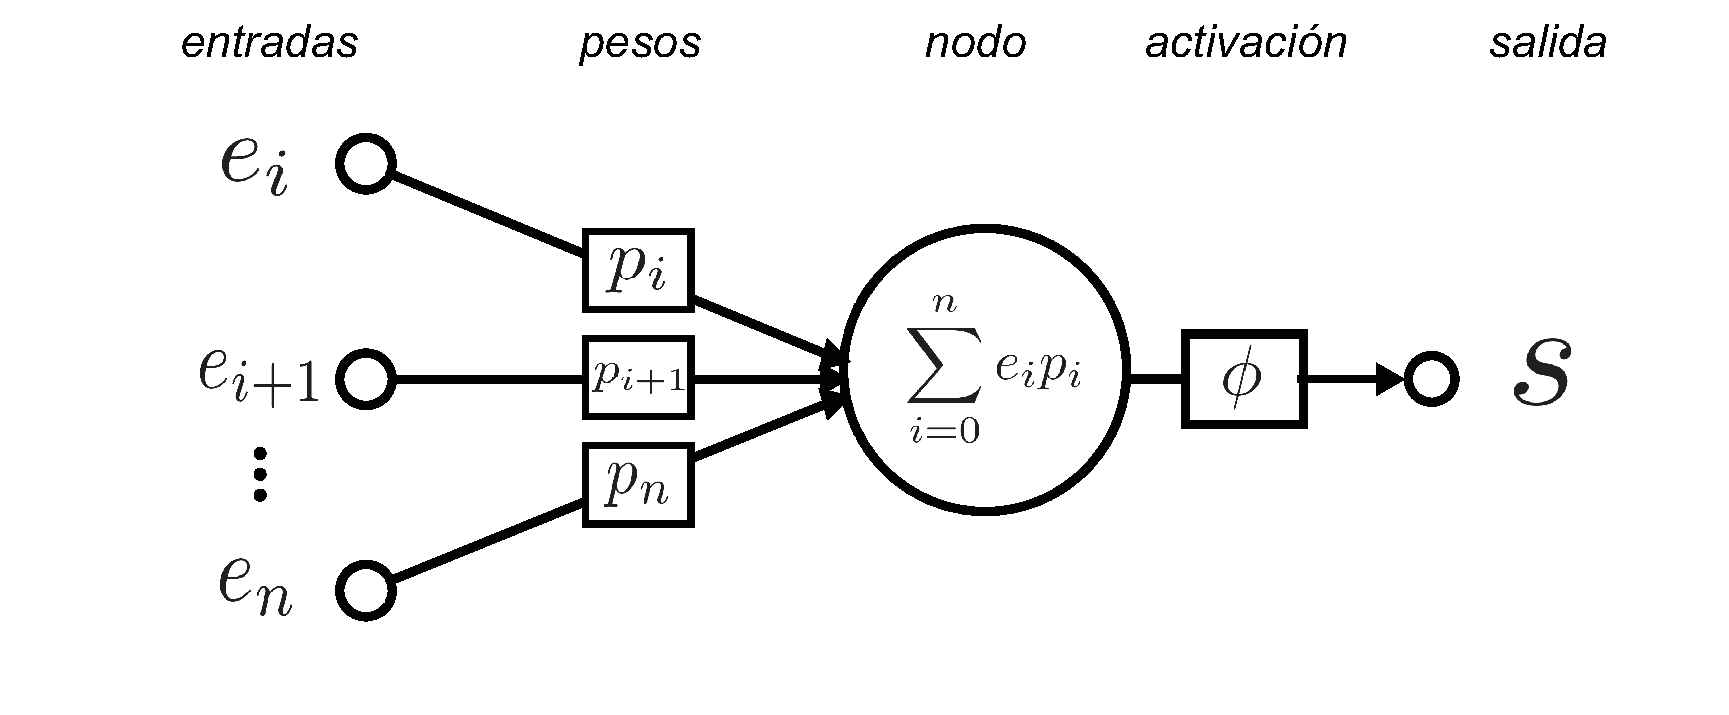
\includegraphics[width=100mm]{Figuras/neural_network.eps}
    \centering
    \caption{Ejemplo de un perceptrón.}
    \label{fig:percep}
\end{figure}

Partiendo de lo anterior, creando arreglos con estos nodos podemos formar estructuras denominadas \emph{redes neuronales}, las cuales cuentan con los siguientes elementos estructurales:

\begin{description}
    \item[Capa de entrada (\emph{input layers})] { Se trata de la primera capa del modelo, en el caso de imágenes a cada pixel le corresponde un nodo de entrada. Estos nodos deben tener las mismas dimensiones que las imágenes de entrada.}
    \item[Capa oculta (\emph{hidden layer})] {Las dimensiones de estos nodos pueden ser diferentes a los de entrada y tener varias capas ocultas, sin embargo esto puede afectar la complejidad y precisión del modelo.} 
    \item[Capa de salida (\emph{output layer})]  {Esta es la capa de salida del modelo, las dimensiones de la capa de salida determinan las dimensiones del dato resultante}
    \item[Función de activación (\emph{activation})]{Se trata de una función dentro de cada nodo que interactúa con el valor entrante y se multiplica por el peso.}
    \item[Pesos (\emph{weight})] {Se trata de un valor entre el nodo de la capa actual y el nodo siguiente inicializado de forma aleatoria y después ajustado por un algoritmo para aproximar la salida al valor real.}  
    \item[Sesgo (\emph{bias})] {Se trata de un valor constante que se suma al resultado de la función de activación y el peso, de esta forma se puede ajustar que tan fácil o difícil es activar un nodo.} 
\end{description}

\subsection{Evaluación y Optimización}
Para realizar el proceso de \emph{aprendizaje} del modelo, primero se debe evaluar cuál es el estado actual de las predicciones. Para esto es necesario evaluar que distancia existe entre el valor predicho y el valor real, esto se puede lograr mediante una \emph{función de pérdida} que se encargue de determinar que tanta diferencia (\emph{loss}) existe en las estimaciones del modelo con los pesos actuales.

Un ejemplo de la función de pérdida es el de la función logarítmica del costo (\emph{log-likelihood}), como se muestra a continuación
\begin{equation}
    l(\mathbf{y}, \hat{\mathbf{y}}) = - \sum_{j=1}^q (y_j \log \hat{y}_j),     
\end{equation}
$q$ representa el número de clases entre las cuales predecir, $y_j$ representa el valor de salida real, $\hat{y_j}$ el valor estimado de salida por el modelo y $j$ la posición indizada de clase.

Ya que se tiene calculada la pérdida del modelo en su configuración de pesos actual, es necesario actualizar el valor de todos los pesos dentro del modelo para poder acercarnos al valor real. Aquí es donde participa el algoritmo de \emph{gradiente descendiente} \citep{alg:gradient}, dicho algoritmo se puede representar con la siguiente ecuación
\begin{equation}
        \text{error} = \frac{\partial}{\partial m} = \frac{2}{N}\sum_{i=1}^{N}-X_i(y_i-(mX_i+b)),
\end{equation}
\begin{equation}
        \frac{\partial}{\partial b} = \frac{2}{N}\sum_{i=1}^{N}(y_i-(mX_i+b)),
\end{equation}
donde $m$ y $b$ son valores enteros que representan el peso de dos parámetros de un modelo, los cuáles serán optimizados para acercar la salida del modelo a la salida real.

%\begin{algorithm}
%    \begin{algorithmic}
%        \For{$k = 0, 1 , 2 \dots n$}{
%
%            $g_k \leftarrow \nabla f(x_k)$ 
%           
%            $x_{k+1} \leftarrow x_k - t_k g_k$
%            }
%    \end{algorithmic}
%\end{algorithm}


\chapter{Estado del Arte}
En este capítulo se estudia las literaturas relacionadas con el presente trabajo de tesis con el objetivo de hacer una comparativa entre distintos métodos para resolver el mismo problema, o implementaciones similares para resolver problemas distintos.

En la primera sección, \emph{trabajos similares}, se recopilan trabajos con características relacionadas al presente trabajo de tesis, ya sea relacionados con el método o con el problema que se pretende resolver, se describe el tema que abarcan y los puntos que lo relacionan con el trabajo aquí presente.

En la segunda sección, \emph{análisis comparativo}, se comparan las distintas características de los trabajos revisados, de esta forma podemos determinar las principales diferencias así como las ventajas y desventajas de cada trabajo. Así mismo se recopilaran todas estas diferencias en una tabla para visualizar mejor estas características.

Finalmente en las \emph{áreas de oportunidad}, se realiza una conclusión acerca de los resultados en la tabla comparativa.

\section{Trabajos Similares}

A continuación se mencionan los trabajos revisados en los que se puede obtener un punto de convergencia ya sea en los métodos similares utilizados para resolver problemas diferentes o en su defecto métodos distintos para resolver problemas similares.

\citet{DBLP:journals/corr/BadrinarayananK15} en este se describe la arquitectura denominada \texttt{SegNet} utilizada principalmente para la conducción autónoma y la detección de peatones, se describe como una arquitectura convolucional, con la característica de que es una jerarquía de codificador-decodificador donde a cada codificación (\emph{encoding}) corresponde una capa de agrupación de máximos (\emph{max pooling}) y un decodificador. Inspirado principalmente en la arquitectura \texttt{VGG16}, con la diferencia de que el componente clave en esta arquitectura es el uso de convoluciones en lugar de la capa completamente conectada de nodos (\emph{fully-connected-layer}) a la salida.

\citet{DBLP:journals/corr/RonnebergerFB15} proponen uno de los primeros modelos de la redes neuronales convolucionales denominada \texttt{U-net} dirigida al análisis de imágenes del area médica. Este trabajo consiste en una arquitectura con dos trayectorias: la trayectoria de contracción de la imagén y la trayectoria de expansión. En la trayectoria de contracción de la imagen se aplica una secuencia de convoluciones de dimension $3 \times 3$ con solapado, seguido de una función de activación de rectificación linear unitaria (ReLu) y posteriormente una operación de agrupación de máximos (\emph{max pooling}) para la compresión de la imagen (\emph{downsampling}). Por otro lado, la trayectoria de expansión consiste de el escalado de la imagen (\emph{upsampling}), en cada paso se aplica una capa de convolución de $2 \times 2$ a la cuál se concatena una imagen recortada del mapa de características de la trayectoria de contracción y dos convoluciones de $3 \times 3$ seguidos de una activación ReLu cada una. En total la arquitectura tiene 23 convoluciones (U-net).

\citet{DBLP:journals/corr/ChenPK0Y16} en este trabajo describen la arquitectura denominada \texttt{Deep Lab}, la cual propone un acercamiento distinto a la parte de la reconstrucción en las capas finales del modelo. Al igual que otras arquitecturas cuenta con capas de convolución. agrupación de máximos y activación de rectificación linear unitaria, sin embargo, el componente clave aquí es la denominada convolución de hoyos (\emph{atrous convolution}), la cual es una modificación al filtro de convolución basado en la transformada de \emph{Wavelet} para el escalado del mapa de características (\emph{upsampling}). De esta forma se obtiene una alternativa al uso de capas de deconvolución y así se aumenta la resolución del mapa de características a la salida del modelo sin aumentar el tiempo de computación o la cantidad de parámetros.

\citet{DBLP:journals/corr/TeichmannWZCU16} reducen la carga computacional en los modelos de redes neuronales convolucionales mediante la unificación de las tres tareas principales de estas: clasificación, detección y segmentación. Denominada como multi-red neuronal \texttt{MultiNet} se trata de una arquitectura tipo codificador-decodificador en donde el decodificador esta compuesto de tres ramas las cuales corresponden a las tareas de clasificación, detección y segmentación por lo que se realizan las tres tareas de forma simultanea partiendo de la misma entrada (\emph{multi-tasking}) y usando la salida de cada una de las ramas para el ajuste fino de los parámetros del modelo (\emph{fine-tuning}).  

\citet{KRONER2020261} describen un modelo de codificación-decodificación contextual basado en el proceso en el que los humanos obtenemos la información espacial de los escenarios visuales complejos, mediante un mapa topográfico de las salientes. Se basa en más en el proceso biológico con el que se obtiene la información espacial que en los métodos matemáticos para calcularla, dicho lo anterior, los principales componentes para determinar una saliente son color, la intensidad y la orientación.  

\citet{KADAMPUR2020100282} proponen el úso de los servicios de nube en conjunto con las redes neuronales profundas y el diseño de modelos utilizando modelos pre-entrenados. Para esto utilizan la herramienta de \texttt{Deep Learning Studio}, la cual es un software que permite el uso de tarjetas gráficas (\emph{GPU}) localizadas en la nube o localmente, y también permite el uso de múltiples tarjetas de forma simultanea (\emph{multi-GPU}), la arquitectura usada para la detección de cáncer de piel en este trabajo es de una red neuronal profunda de clasificación, por lo que el modelo se codifica mediante convoluciones y se decodifica mediante capas de aplanamiento (\emph{flatten layer}) para posteriormente entrar a una capa de nodos completamente conectada (\emph{fully-connected-layer}) y obtener dos posibles resultados: es cáncer o no es cáncer.

\citet{zhou2019emerging} hablan sobre el aprendizaje de máquina \texttt{Machine Learning} y las redes neuronales para la predicción teórica de nano-materiales. Primero determinaron el número de capas y la heterogeneidad del material para posteriormente entender los fenómenos visuales como el parpadeo y la emisión cuántica, concluyendo que las intensidades RGB están correlacionadas al número de capas en el material del grafeno. 

\citet{DBLP:journals/corr/LucCCV16} proponen una alternativa al proceso de decodificación. Normalmente en las tareas de segmentación es necesaria la parte de codificación para realizar las predicciones a grado pixel y la decodificación para reconstruir la imagen con las categorías segmentadas. Este trabajo propone el uso de una red generativa adversaria \texttt{GAN}, para utilizarse como decodificador, de esta manera se obtiene un mapa de etiquetas (\emph{map layer}) con una mayor resolución.

\citet{JAIN2015735} desarrollan una herramienta de procesamiento de imágenes médicas relacionadas al melanoma, basándose en sus características físicas como: asimetría, color, bordes y diámetro. Se basa en la técnica de segmentación de imágenes mediante el uso de filtros de contraste, detección de ejes, etc. A diferencia de los otros trabajos mencionados, este no consiste del uso de redes neuronales sino de filtrados de imágen mediante distintos kernels de convoluciones para obtener la máscara.

\section{Análisis Comparativo}
En esta sección se evalúan los trabajos revisados con el trabajo propuesto en este trabajo de tesis, para esto se define una serie de características que servirán como puntos de referencia entre el trabajo propuesto y los trabajos relacionados, dichas características son las siguientes:

\begin{description}
    \item[Modelo]{Tipo de arquitectura del modelo.}
    \item[Clasificación]{El sistema puede clasificar entre distintas categorías.}
    \item[Segmentación]{El sistema puede segmentar las imágenes.}
    \item[Supervisado]{ El sistema requiere de datos de datos de entrenamiento.}
    \item[Pre-entrenamiento]{El sistema puede inicializarse con pesos pre-entrenados como alternativa a la inicialización con pesos aleatorios.}
    \item[Evaluación]{El sistema cuenta con una función de evaluación y un algoritmo de optimización.}
    \item[Salida]{Características de los datos obtenidos en la salida del modelo.}
\end{description}
\newpage
\begin{table}[hbt!]{
    \centering
    \caption{Similitudes y diferencias entre los trabajos revisados; las características implementadas se representan con \cmark, mientras que las no implementadas con \xmark.}
    \begin{adjustbox}{width=\textwidth}
        \begin{tabular}[t]{|l|l|l|l|l|l|l|l|}
            \hline
            \bf{Trabajo} & \bf{Modelo} & \rotatebox{90}{Clasificación} & \rotatebox{90}{Segmentación} & \rotatebox{90}{Supervisado} & \rotatebox{90}{Pre-entrenamiento\phantom{m}} & \rotatebox{90}{Evaluación} & Salida\\
            \hline
            \citet{DBLP:journals/corr/BadrinarayananK15} & \texttt{SegNet} & \cmark & \cmark & \cmark & \cmark & \cmark & mapa de etiquetas\\
            \citet{DBLP:journals/corr/RonnebergerFB15} & \texttt{U-net} & \cmark & \cmark & \cmark & \xmark & \cmark & mapa de etiquetas\\
            \citet{DBLP:journals/corr/ChenPK0Y16} & \texttt{DeepLab} & \cmark & \cmark & \cmark & \xmark & \cmark & mapa de etiquetas\\   
            \citet{DBLP:journals/corr/TeichmannWZCU16} & \texttt{MultiNet} & \cmark & \cmark & \cmark & \xmark & \cmark & mapa de etiquetas\\   
            \citet{KRONER2020261} & \texttt{VGG16} & \cmark & \cmark & \cmark & \cmark & \cmark & mapa de calor\\ 
            \citet{KADAMPUR2020100282} & \texttt{CNN} & \cmark & \xmark & \cmark & \xmark & \cmark & mapa de etiquetas\\    
            \citet{zhou2019emerging} & \texttt{ML / SVM} & \cmark & \xmark & \cmark & \xmark & \cmark & etiqueta\\    
            \citet{DBLP:journals/corr/LucCCV16} & \texttt{CNN/GAN} & \cmark & \cmark & \cmark & \cmark & \cmark & mapa de etiquetas\\         
            \citet{JAIN2015735} & \texttt{A.B.C.D} & \xmark & \cmark & \xmark & \xmark & \xmark & etiqueta\\
            \hline
            Propuesta de tesis & \texttt{FPN} & \cmark & \cmark & \cmark & \cmark & \cmark & mapa de etiquetas\\
            \hline   
        \end{tabular}
    \end{adjustbox}
    \label{Tab:comp_1}}
\end{table}

\newpage

\section{Áreas de Oportunidad}
En esta sección se señalan las características de los trabajos mencionados en la sección anterior y se compara con las características del método propuesto en este trabajo de tesis para obtener una comparativa sobre las áreas de oportunidad.

Para las tareas de segmentación es fundamental contar con un codificador y un decodificador eficientes, sin embargo aún más importante es tener la capacidad de evaluarse así mismo y optimizarse, a diferencia de algunas técnicas más robustas de diseño, las redes neuronales convolucionales permiten esas funcionalidades. Otro aspecto importante a considerar es la capacidad del úso de pesos pre-entrenados a la hora de entrenar utilizando nuestros datos, ya que incluso cuando los pesos pre-entrenados fueron obtenidos mediante bases de datos no necesariamente relacionadas con el o los objetos que nosotros queremos detectar, pero con similitudes físicas, en teoría ofrece un mejor desempeño y reduce el tiempo de entrenamiento ya que de lo contrario, se tendría que inicializar el modelo con pesos distribuidos de forma aleatoria, por lo que la precisión inicial del modelo sería cercana al cero por ciento. En este trabajo de tesis, el modelo propuesto cuenta con la capacidad de utilizar pesos pre-entrenados, el reto está en seleccionar un conjunto de pesos que mejoren la precisión en el caso de imágenes médicas, ya que si los pesos utilizados fueron obtenidos con imágenes que difieren mucho de las imágenes que se utilizadas en el presente trabajo, podría verse comprometida la precisión o el tiempo de entrenamiento.

\chapter{Solución Propuesta}
El objetivo de este trabajo de tesis es implementar una técnica para la clasificación y segmentación de regiones de tumores del tipo melanoma en imágenes dermatolólogicas mediante el úso del aprendizaje profundo (\emph{deep learning}). Para comprobar la hipótesis se desarrolló una aplicación de software cuya función es la de funcionar como entorno de trabajo mediante el cuál se puedan procesar datos para el entrenamiento de modelos, trabajar con distintas arquitecturas de redes, así como modificar los parámetros del entrenamiento para hacer el ajuste fino del modelo.

En este capítulo se describe la estructura de la implementación propuesta, comenzando con la \emph{metodología}, en donde se describe el conjunto de procedimientos por los cuales debe atravesar los datos desde su entrada como una imagen ya sea de un canal o triple canal, hasta su salida como máscara de segmentación con sus respectivas regiones clasificadas a su categoría correspondiente. Posteriormente en \emph{implentación de la solución} se describe el lenguaje utilizado para la implementación, las librerías utilizadas; así como el análisis llevado a cabo para determinar cuál configuración de parámetros ofrece el mejor resultado y una comparativa o \emph{benchmarking}.

\section{Metodología}
La herramienta propuesta cuenta con tres fases principales:cargado y filtrado de datos, entrenamiento y predicción, la fase de \emph{cargado de datos} consiste en adquirir y corregir las imágenes que serán usadas en las fases siguientes, el \emph{entrenamiento} trata de la obtención de un modelo a partir de dos datos: la imagen real (entrada) y la máscara conocida (salida deseada) que corresponde a la región a clasificar, el proceso de entrenamiento consta de un número determinado de ciclos también denominados épocas (\emph{epochs}) en dónde se prueban distintas configuraciones y se conserva la configuración con el mayor porcentaje de precisión. Al finalizar el entrenamiento se obtiene un modelo mediante el cuál se realiza la segunda fase, \emph{predicción}, ahora únicamente se requiere un dato de entrada el cuál es la imágen de la cual se desconoce la clasficación de sus regiones, y como resultado se obtiene una estimación de la máscara de segmentación desconocida con sus regiones correctamente clasificadas.

\tikzstyle{decision} = [diamond, draw, fill=gray!20, 
    text width=5.5em, text badly centered, node distance=3cm, inner sep=0pt]
\tikzstyle{block} = [rectangle, draw, fill=gray!20, 
    text width=8em, text centered, rounded corners, minimum height=4em]
\tikzstyle{line} = [draw, -latex']
\tikzstyle{cloud} = [draw, ellipse,fill=red!20, node distance=3cm,
    minimum height=2em]

\begin{figure}[b]
\centering    
\begin{tikzpicture}[node distance = 4.5cm, auto]
    % Nodos.
    \node [block] (init) {Cargado y Filtrado de Datos};
    \node [block, right of = init] (train) {Entrenamiento del Modelo};
    \node [block, right of = train] (pred) {Predicción de Máscaras};
    % Ejes.
    \path [line] (init) -- (train); 
    \path [line] (train) -- (pred); 
\end{tikzpicture}
\caption{Diagrama de flujo general de la herramienta propuesta.}
\end{figure}


\subsection{Características de los Datos de Entrada}
Para poder llevar a cabo la creación del modelo primero es necesario tener un conjunto de datos (\emph{dataset}) que será utilizado para el entrenamiento y la validación de la configuración de pesos sinápticos en la época presente.
A partir de éste momento se referirá como \emph{muestra} al conjunto de datos de entrada del entrenamiento del modelo; como se mencionó al comienzo del capítulo, para llevar a cabo el entrenamiento es necesario otorgar al sistema dos entradas: la imagen real y la máscara conocida de las regiones ya clasificadas. Por lo tanto una muestra es el equivalente a la concatenación de una imágen dermatolólogica y la máscara conocida correspondiente. Con una sola muestra se puede generar un modelo sin embargo la precisión sería muy baja, generalmente entre mayor sea la cantidad de muestras se puede obtener una mejor precisión. No obstante depende mucho de la variabilidad de las imágenes, ya que si se tratara de entrenar un modelo de muchas categorías, la variabilidad haría mas complejo el modelo y por ende requiriría de un mayor número de épocas para alcanzar una precisión viable (\emph{underfit}); así como el úso de un \emph{dataset} muy extenso de pocas categorías y con imágenes muy similares podría causar justamente lo contrario (\emph{overfit}), lo cuál no permitiría realizar predicciones correctamente en imágenes no tan parecidas a las usadas en el entrenamiento.

\subsection{Codificación de Características}
Para poder realizar una predicción de la máscara segmentada, primero es necesario reducir las dimensiones de las imágenes sin afectar la información que estas representan. Para conseguir esto se utiliza un filtro de \emph{convolución de matríces}. Una imágen es una función bidimensional $ z = f(x,y)$, donde $x$ y $y$ son coordenadas espaciales y $z$ es el valor de la intensidad de la imágen en el punto $(x , y)$, en el caso de las imágenes a color se tienen tres funciones donde cada una representa la intensidad del pixel del canal correspondiente (rojo, verde o azul) \citep[~p. 100]{conv_1}. La convolución de matríces se define como la obtención de una matríz $C$ a partir de dos matríces $A$ y $B$. La matríz $A_{m \times n}$ sería el mapa de intensidad de pixeles de la imágen mientras que la matríz $B_{(2N+1) \times (2N+1)}$ es el kernel de la convolución, mediante la ecuación \ref{eq:conv_1} se obtiene la matríz $C = A * B$
\begin{equation}
c_{ij} = \frac{1}{b} \sum_{r=1}^{2N+1}\sum_{s=1}^{2N+1}(a_i-N+r-1, i-N+r-1),
\label{eq:conv_1}
\end{equation}
donde $b = \sum_{i,j=1}^{2N+1} b_{i,j}$, si $b=0$ se toma $b=1$.

\begin{figure}[b]
    \centering
    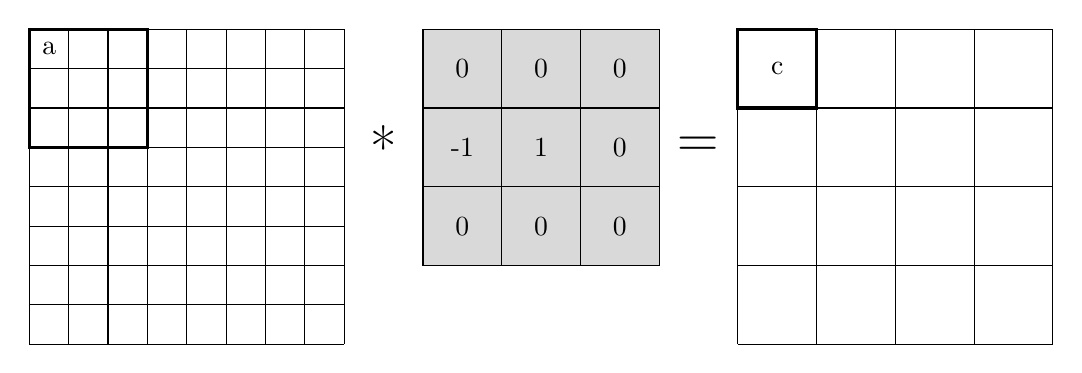
\begin{tikzpicture}
        \draw[step=0.5cm, black, thin](0,0) grid (4,4);
        \node (a_in) at (0.25, 3.75) {a};
        \filldraw[fill = gray!30, draw = black] (5,1) rectangle (8,4);
        \draw[step=1cm, black, thin](5,1) grid (8,4);
        \draw[step=0.5cm, black, line width=0.40mm](0,4) rectangle (1.5, 2.5);
        \node (ast) at (4.5, 2.5) {\huge *};
        \node at (5.5,3.5) {0};
        \node at (5.5,2.5) {-1};
        \node at (5.5,1.5) {0};
        \node at (6.5,3.5) {0};
        \node at (6.5,2.5) {1};
        \node at (6.5,1.5) {0};
        \node at (7.5,3.5) {0};
        \node at (7.5,2.5) {0};
        \node at (7.5,1.5) {0};
        \node (eq) at (8.5, 2.5) {\huge =};
        \draw[step=1cm, black, thin](9,0) grid (13,4);
        \filldraw[fill=white, draw=black, line width=0.40mm](9,4) rectangle (10,3);
        \node (c_out) at (9.5,3.5) {c};  
    \end{tikzpicture}
    \caption{Representación del proceso de obtención de la matriz convolucionada.}
\end{figure}

El filtro de convolución es la base del proceso de codificado de la imagen, la codificación se refiere a la transformación de una imagen a un vector de características de alta dimensión (\emph{downsampling}), una vez que se tiene el mapa de características sigue con el proceso de \emph{upsampling}.

\subsection{Modelo FPN}
La arquitectura de red neuronal tipo red piramidal de características, por sus siglas en inglés FPN\footnote{FPN: Feature Pyramid Network}, se trata de una estructura que funciona en conjunto con el codificador \texttt{ResNet}, mientras el codificador tiene la tarea de realizar el \emph{downsampling} de las dimensiones espaciales de la imágen de entrada y convertirlas a un mapa de característica , el decodificador hace justamente lo opuesto (\emph{up-sampling}), a partir del mapa de características producto de la codificación, realiza una secuencia de deconvoluciones que construyen la máscara de segmentación estimada.

\begin{figure}[h]
    \centering
    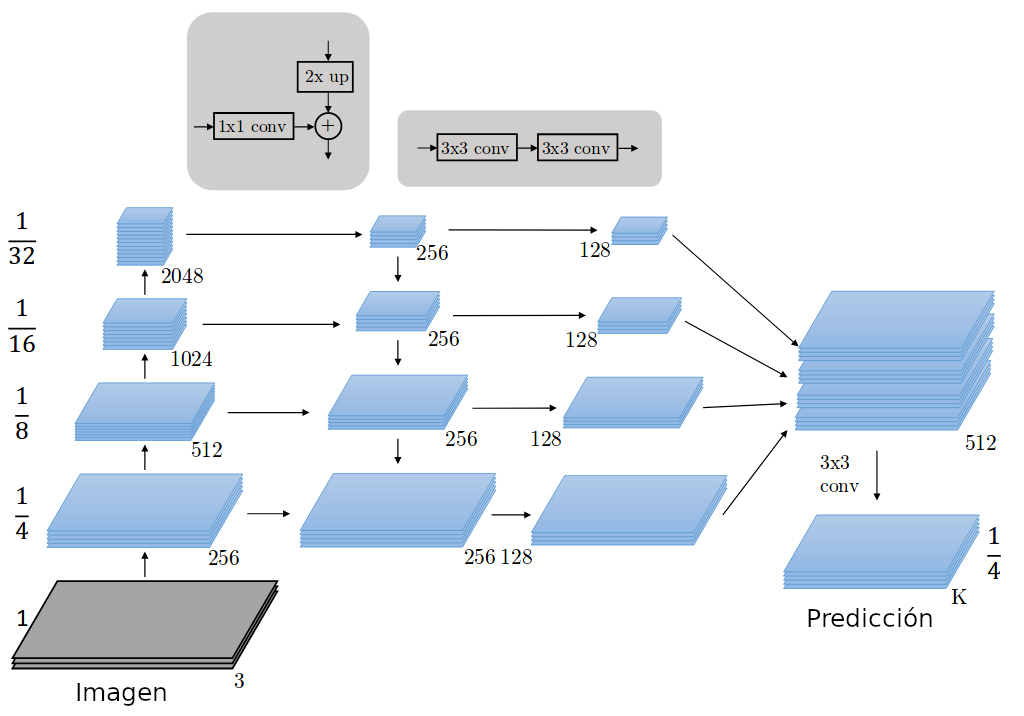
\includegraphics[scale=0.55]{Figuras/fpn_ar_esp.png}
    \caption{Representación de la arquitectura FPN \citep{fpn_2}.}
    \label{fig:fpn_map}
\end{figure}
\coltext{corregir $\times$}

En la figura \ref{fig:fpn_map} se puede apreciar la arquitectura y la transformación de las dimensiones de los datos, el número a lado izquiero de las capas de convolución representa la resolución en proporción a la entrada y el número de lado derecho representa el número de canales. El número de canales aumenta mientras que la resolución disminuye.

\section{Implementación de la Solución}
Para la implementación de la herramienta propuesta, se utilizó \texttt{Python} como lenguaje principal. \texttt{Python} es un lenguaje de alto nivel con un extenso repositorio de paquetes desarrollados por la comunidad, también es un lenguaje ligero ideal para el procesamiento de datos y de operaciones con datos de altas dimensiones (\emph{high-dimensional data}), debído a esto último, se consideró \texttt{Python} la mejor opción para la implementación de la red neuronal profunda.

Si bien otros lenguajes tienen una mayor velocidad en la ejecución de cálculos complejos, es la facilidad con la que se pueden desplegar implementaciones complejas en relativamente pocas líneas de código lo que llevo a la conclusión de que \texttt{Python} es la opción ideal para la implementación propuesta, como el hecho de que existen muchas documentaciones e implementaciones similares en este lenguaje.

A continuación se especifican las librerías claves utilizadas para llevar a cabo la implementación, así mismo se da una breve descripción general sobre la misma y su importancia durante el desarollo de la propuesta.

\begin{table}[H]
    \centering
    \caption{Librerías utilizadas para la implementación de la propuesta.}
    \scalebox{0.90}{
    \begin{tabular}{|p{3cm}|p{10cm}|}
        \hline
        \bf{Librería} & \bf{Descripción} \\
        \hline
        \texttt{Torch.vision} & Este paquete es una colección de módulos relacionados con las operaciones de tensores y la aceleración de cálculos mediante hardware. Se usa en conjunto con \texttt{NumPY} y cuenta con las arquitecturas de redes neuronales típicas, así como herramientas para el cargado de datos y la configuración de parametros de los modelos.\\
        
        \hline
        \texttt{Quvel Segmentation Models} & Este paquete cuenta las arquitecturas de las redes neuronales de segmentación semántica típicas, se trata del marco de trabajo mediante el cuál podemos crear y configurar la arquitectura de la red para después realizar el entrenamiento.\\
        
        \hline
        \texttt{Numpy} & Esta librería fue desarrollada para habilitar el uso de vectores y matríces de grandes dimensiones y para la computación numérica en general, ya que \texttt{Python} originalmente no cuenta con el soporte para esto.\\
        
        \hline
        \texttt{OpenCV} & Es una librería dedicada al procesamiento de imágenes y a la visión computacional, cuenta con funciones que permiten cargar imágenes y obtener su matríz de pixeles así como aplicar efectos y transformaciones en estas.\\

        \hline
        \texttt{Albumentations} & Esta librería es principalmente útil para el pre-procesado de las imágenes al momento de realizar el entrenamiento, cuenta con funciones que permiten crear secuencias de transformaciones específicas para distíntos subconjuntos de datos así como la capacidad de transformar imágenes a tensores.\\

        \hline
    \end{tabular}}
    \label{tab:libs}
\end{table}

En el cuadro \ref{tab:specs} se especifícan las características del equipo en el cuál fue realizado el experimento.

\begin{table}[H]
    \centering
    \caption{Especificaciones técnicas de los componentes.}
    \begin{tabular}{|l|l|}
        \hline
        \bf{Componente} & \bf{Descripción} \\
        \hline
        CPU & AMD Ryzen 5 3600x, 3.80 GHz, de seis núcleos.\\
        \hline
        GPU & Nvidia GeForce 1050ti, 4 GB. \\
        \hline
        RAM & HyperX Fury, 16 GB, 2433 MHz. \\
        \hline
        Tarjeta Madre & Gigabyte Gaming AB-350. \\
        \hline
        Sistema Operativo & Ubuntu 20.4 \\
        \hline
    \end{tabular}
    \label{tab:specs}
\end{table}
\subsection{Computación Asistída por Hardware}
Los cálculos llevados en el proceso de entrenamiento involucran realizar operaciones con datos de altas dimensiones (\emph{high-dimensional data}) los cuales requieren una gran cantidad de recursos de procesamiento, estas operaciones al estar relacionadas con vectores y matríces pueden ser ejecutadas rapidamente por la unidad GPU\footnote{GPU: Graphics Processor Unit}, entre mayor sea la velocidad de procesamiento de la GPU más rápido es el entrenamiento de nuevos modelos y con mayor resolución.

\subsection{Módulos de la Implementación}
La herramienta desarrollada en el presente trabajo de tesis se divide en cuatro módulos funcionales y un módulo central encargado de controlar la ejecución de los mismos. En la figura \ref{fig: modules} se puede observar la estrúctura modular del software desarrollad, dentro de dichos módulos se encuentran las funciones específicas de esa categoría y en el módulo principal se encuentran los parámetros del modelo.

\tikzstyle{block} = [rectangle, draw, fill=gray!20, 
    text width=7em, text centered, minimum height=4em]
\tikzstyle{line} = [draw, -latex']
\tikzstyle{cloud} = [draw, ellipse,fill=red!20, node distance=3cm,
    minimum height=2em]

\begin{figure}[H]
    \centering
    \begin{tikzpicture}[node distance = 1cm and 1cm]
        \node [block] (main) {main};
        \node [block, left= of main] (load) {load$\_$dataset};
        \node [block, right= of main] (train) {train$\_$model};
        \node [block, below= of main] (test) {test$\_$model};
        % Líneas
        \path [line] (load) -- (main);
        \path [line] (train) -- (main);
        \path [line] (test) -- (main);
    \end{tikzpicture}
    \caption{Distribución de los módulos en la herramienta desarrollada.}
    \label{fig: modules}
\end{figure}

\subsection{Lectura de Entrada}
El proceso de cargado de datos y filtrado es un proceso muy importante para la ejecución correcta en las siguientes transformaciones, para el entrenamiento del modelo se utilizará una base de datos obtenida de la Asociación de Recolección de Imágenes dermatolólogicas, por sus siglas en inglés (\emph{ISIC}\footnote{ISIC: International Skin Imaging Collaboration.}). La base de datos de ISIC cuenta con diez mil imágenes de entrenamiento con resoluciones distintas, con diferentes tonos de iluminación y rotación, así como su máscara de segmentación conocida y dos mil imágenes para realizar pruebas, también con resoluciones no estandarizadas y sin máscara de segmentación.

\definecolor{folderbg}{RGB}{124,166,198}
\definecolor{folderborder}{RGB}{110,144,169}

\def\Size{4pt}
\tikzset{
  folder/.pic={
    \filldraw[draw=folderborder,top color=folderbg!50,bottom color=folderbg]
      (-1.05*\Size,0.2\Size+5pt) rectangle ++(.75*\Size,-0.2\Size-5pt);  
    \filldraw[draw=folderborder,top color=folderbg!50,bottom color=folderbg]
      (-1.15*\Size,-\Size) rectangle (1.15*\Size,\Size);
  }
}
\begin{figure}[H]
    \centering
    \begin{forest}
        for tree={
          font=\ttfamily,
          grow'=0,
          child anchor=west,
          parent anchor=south,
          anchor=west,
          calign=first,
          inner xsep=7pt,
          edge path={
            \noexpand\path [draw, \forestoption{edge}]
            (!u.south west) +(7.5pt,0) |- (.child anchor) pic {folder} \forestoption{edge label};
          },
          before typesetting nodes={
            if n=1
              {insert before={[,phantom]}}
              {}
          },
          fit=band,
          before computing xy={l=15pt},
        }  
      [Data
        [Train$\_$Images
        ]
        [Annot$\_$Images
        ]
        [Test$\_$Images
        ]
      ]
      \end{forest}
      \caption{Representación del árbol de directorios de imágenes.}    
\end{figure}


Lo primero que se desarrolló fue un asistente de cargado y filtrado de imágenes, en el código \ref{code:load} se puede apreciar el código fuente y las funciones utilizadas para tal motivo. Al ser utilizado el objeto \emph{dataset} y alimentar los argumentos con los directorios de las imágenes se obtiene como resultado un objeto de dimensión $N \times 2 \times (m \times n)$ donde $N$ es el número de muestras cargadas y el primer elemento de la fila es la matríz de la imágen real, y el segúndo la matríz de la máscara conocída.

\renewcommand{\lstlistingname}{Código}
\definecolor{codegreen}{rgb}{0,0.6,0}
\definecolor{codeblue}{rgb}{0.121, 0.203, 0.858}
\definecolor{codegray}{rgb}{0.5,0.5,0.5}
\definecolor{codepurple}{rgb}{0.58,0,0.82}
\definecolor{backcolour}{rgb}{0.95,0.95,0.92}

\lstdefinestyle{pystyle}{
    basicstyle=\linespread{0.8},
    backgroundcolor=\color{backcolour},   
    commentstyle=\color{codegreen},
    keywordstyle=\color{codeblue},
    numberstyle=\tiny\color{codegray},
    stringstyle=\color{codepurple},
    basicstyle=\ttfamily\footnotesize,
    breakatwhitespace=false,         
    breaklines=true,                 
    captionpos=b,                    
    keepspaces=true,                 
    numbers=left,                    
    numbersep=5pt,                  
    showspaces=false,                
    showstringspaces=false,
    showtabs=false,                  
    tabsize=2
}
\lstset{style=pystyle}
\begin{lstlisting}[language = Python, label = {code:load} ,caption= Código fuente del asistente de cargado de imágenes.]
    # load_dataset.py
    class dataset ():
        def __init__(self, images_dir, masks_dir, classes=None,):
        # Extraccion de ids de imagenes y mascaras.
        self.ids = listdir(images_dir)
        self.images_fps = [os.path.join(images_dir(img_id)
                          for img_id in self.ids]
        self.masks_fps = [os.path.join(mask_dir,
                         (img_id[:-4] + '_segmentation.png'))
                         for img_id in self.ids]
    # Lectura de imagenes y correcion de canales.
    def __getitem__(self,i):
        image = cv2.imread(self.images_fps[i])
        image = cv2.cvtColor(image, cv2.COLOR_BGR2RGB)
        mask = cv2.imread(self.masks_fps[i],0)
        return image, mask
\end{lstlisting}

\begin{lstlisting}[language = Python, label = {code:load_2} ,caption= Invocación de la función contenida dentro de la clase.]

    # main.py.
    import load_dataset as ld 
    train_dir = 'Data/Train_Images'
    mask_dir = 'Data/Train_Images'
    set_de_datos = ld.dataset(train_dir, mask_dir)
    # Al indicar la posicion dentro del dataset se obtiene una muestra dividida en dos objetos:
    imagen, mascara = set_de_datos[1]

\end{lstlisting}

En el código \ref{code:load_2} se invoca la función \texttt{dataset}, la cuál tiene por argumento la dirección de las imágenes reales y las máscaras conocidas, con esto se crea el conjunto de datos que posteriormente es utilizado en la sección de entrenamiento.


\subsection{Pre-procesamiento}
El \emph{pre-procesamiento} se define como una secuencia de transformaciones que se aplican al momento previo del entrenamiento y afecta a un subconjunto específico de los datos. Para el diseño de la secuencia de transformaciones tanto para el subconjunto de entrenamiento como el subconjunto fueron consideradas las siguientes características.

\begin{description}
    \item[Resolución]{ El codifícador admite resoluciones específicas, debído a las dimensiones admitidas para el filtrado de convolución de matríces.}
    \item[Número de muestras]{La cantidad de datos disponibles para el entrenamiento afecta la precisión final, si el conjunto de datos es limitado se pueden realizar transformaciones de las imágenes presentes para obtener más datos de entrenamiento. Así como tener un conjunto muy extenso y con poca variabilidad afectaría también la capacidad de predecir imágenes generalizadas, se puede ajustar mediante el pre-procesamiento.}
    \item[] 
\end{description}


\tikzstyle{block} = [rectangle, draw, fill=gray!20, 
    text width=10em, text centered, minimum height=4em]
\tikzstyle{line} = [draw, -latex']
\tikzstyle{cloud} = [draw, ellipse,fill=red!20, node distance=3cm,
    minimum height=2em]

\begin{figure}[H]
    \centering
    \begin{tikzpicture}[node distance = 0.2cm and -2cm]
        \node [block] (input) {Imagen de Entrada \newline($m \times n$)};
        \node [block, below right=of input] (tr1) {Ajuste de tamaño ($512 \times 512$)};
        \node [block, below right= of tr1] (tr2) {Interpolación (\texttt{\small INTER$\_$AREA)}};
        \node [block, below right= of tr2] (tr3) {Transposición (2, 0, 1)};
        \node [block, below right= of tr3] (out) {Dato de Salida ($N \times (512 \times 512)$)};
        % Líneas
        \path [line] (input) -| (tr1);
        \path [line] (tr1) -| (tr2);
        \path [line] (tr2) -| (tr3);
        \path [line] (tr3) -| (out);
    \end{tikzpicture}
    \caption{Línea de pre-procesamiento.}
    \label{fig: pipeline}
\end{figure}


Debido a que el conjunto de datos es extenso y solo clasifíca entre dos categorías, no es necesario realizar demasiadas trasnformaciones, no obstante es importante trasponer la matríz de entrada para convertir la matríz a tensor.

\subsection{Entrenamiento y Validación}
La secuencia de entrenamiento consiste de un búcle en el cuál se condensan las imágenes en un grupo (\emph{batch}), para ser procesadas por el codificador de forma simultanea, esto para acelerar la velocidad de entrenamiento. Sin embargo, a mayor tamaño de batch también se requiere mayor memoria disponible por la unidad procesadora de gráficos y también la precisión del entrenamiento se ve influenciado. Posteriormente se evalúa mediante el \emph{índice de Jaccard}, como se muestra en la ecuación \ref{eq:jacc}.

\begin{lstlisting}[language = Python, label = {code:train} ,caption= Búcle de entrenamiento. ]

    # Variable inicializada en cero para almacenar la precision maxima obtenida.
    max_score = 0 
    for i in range(0,40):
        print('\n Epoch: {}'.format(i))
        train_logs = train_epoch.run(train_loader)
        valid_logs = valid_epoch.run(valid_loader)

        if max_score < valid_logs['iou_score']:
            max_score = valid_logs['iou_score']
            torch.save(model,('Model/'+encoder+'.pth'))
            print('Highest Score Model Saved: {}'.format(max_score))
        if i == 25:
            optimizer.param_groups[0]['lr'] = 1e-5
            print('decreased decoder learning rate to 1e-5')
     lr= 0.0001),])
\end{lstlisting}

Para poder determinar la eficiencia durante el \emph{entrenamiento} y optimizar los pesos sinápticos es necesario hacer uso de métricas, dichas métricas se aplicarán sobre el subconjunto de validación. Los datos utilizados fueron divididos en una proporción de $70\%$ para entrenamiento y $30\%$ para la validación, el subconjunto de validación no es usado durante el entrenamiento, sino qué, al terminar una época se verifíca con ese subconjunto la precisión.

La librería de Yakubovskiy \citep{Yakubovskiy:2019} cuenta con distintas métricas ya implementadas dentro de su \texttt{API}\footnote{Interfaz de programación por sus siglas en inglés, \emph{Application Programming Interface}.}, dichas métricas se pueden configurar previamente al entrenamiento. En el código \ref{code:metrics} se puede apreciar la selección de la función de métrica, la función de pérdida y el optimizador de pesos del modelo.

La función de pérdida, es la función mediante la cuál se evalúa el error durante el entrenamiento, mediante el dato obtenido del error y el optimizador seleccionado se puede minimizar dicho error.

La métrica, es la función mediante la cuál se evalúa el modelo post-entrenamiento con una función que penaliza más el error que la ecuación utilizada para evaluar el error durante el entrenamiento.

El optimizador, utilizando como referencia el valor de pérdida, determina si es necesario aumentar o disminuir el peso de los nodos entre convoluciones para reducir la pérdida y aumentar la precisión.

\begin{lstlisting}[language = Python, label = {code:metrics} ,caption= Ejemplo de configuración de parámetros. ]
    # main.py.
    import segmentation_models_pytorch as smp
    # Funcion de perdida (Dice Loss)
    loss = smp.utils.losses.DiceLoss() 
    # Metrica de evaluacion (Jaccard Index)
    metric = [smp.utils.metrics.IoU(threshold=0.5),]
    # Funcion optimizadora (Adam)
    optimizer = torch.optim.Adam([dict(params=model.parameters(),
     lr= 0.0001),])
\end{lstlisting}

\subsection{Predicción de Máscaras} 
Una vez obtenido un modelo con precisión buena (\emph{good fit}), el objetivo es generar máscaras desconocidas a partír de las imágenes del set de pruebas. Para esto es necesario popular de nuevo un \emph{dataset} de dimensión $N \times (m \times n)$, básicamente es un vector de matríces donde $N$ es el número de imágenes para realizar la prueba, y $m \times n$ es la resolución de imágen de la cuál se desea obtener la máscara de segmentación.

\begin{lstlisting}[language = Python, label = {code:test} ,caption= Código fuente del modulo de pruebas. ]
    # test_model.py
    def test_model(m_path, t_path, encoder, weights, classes, device):
    # Cargar el modelo generado
    model = torch.load(m_path)
    prep_fn = smp.encoders.get_preprocessing_fn(encoder, weights)
    # Crear el subconjunto de datos para pruebas
    vis_dataset = ds.testing_data(t_path,
    classes,augmentation=tfm.get_validation_augmentation())
    test_dataset = ds.testing_data(t_path,
    classes, 
    augmentation=tfm.get_validation_augmentation(), preprocessing=tfm.get_preprocessing(prep_fn))
    # Seleccionar una muestra al azar.
    n = np.random.choice(len(vis_dataset))
    vis = vis_dataset[n].astype('uint8')
    test_image = test_dataset[n]
    # Realizar una prediccion de mascara con la imagen aleatoria.
    x_tensor = torch.from_numpy(test_image).to(device).unsqueeze(0)
    pred_mask = model.predict(x_tensor)
    pred_mask = (pred_mask.squeeze().cpu().numpy().round())
    #Visualizar la imagen real y la mascara predicha.
    ds.visualize(image=vis, predicted=pred_mask)
\end{lstlisting}

\begin{lstlisting}[language = Python, label = {code:test_2} ,caption= Uso de la función definida en el modulo de pruebas.]
    # main.py
    if test_sample:
    tsm.test_model(model_path, test_dir, ENCODER, ENCODER_WEIGHTS, CLASSES, DEVICE)
\end{lstlisting}

En el código \ref{code:test}, se define la función que se encarga de cargar el modelo y cargar el subconjunto de datos para pruebas mientras que en el código \ref{code:test_2} se da un ejemplo del uso de dicha función. Dando como resultado una gráfica con la imágen de entrada y la máscara estimada para tal.

Con esto finalizarían los procesos de cargado, entrenamiento y predicción de la herramienta propuesta, la línea de transformaciones se diseña en base a la cantidad de datos y las características que estas contienen. A sí mismo dichas transformaciones se llevan a cabo para adaptar las dimensiones de la imagen de entrada con el codificador, posteriormente y durante el entrenamiento se evalúa la configuración de los pesos sinapticos mediante el coeficiente de dados y se optimizan dichos pesos mediante el optimizador \emph{adam}, el cual es una alternativa al método de gradiente descendiente y está diseñado para actualizar los pesos sinápticos en elementos de naturaleza iterativa como es el caso de las imágenes. 



\chapter{Experimentos}
En este capítulo se presentan los experimentos llevados a cabo durante el desarrollo de la herramienta propuesta. Las siguientes secciones corresponden a diferentes experimentos llevados a cabo para validar la hipótesis del presente trabajo de tesis, cada experimento contiene tres subsecciones: \emph{diseño experimental}, \emph{resultados} y \emph{discusión}.

En la subsección de \emph{diseño experimental}, se detalla el experimento y el parámetro que se pretende definir en base a este, todos los procesos realizados por la herramienta desarrollada en el presente trabajo de tesis se ejecutan de forma secuencial, debido a esto es necesario determinar el mejor parámetro en cada paso de la transformación.

En \emph{resultados}, se reporta e interpreta todos los resultados obtenidos mediante el experimento llevado a cabo en esa sección, cada experimento cuenta con su propia sección y se determina el mejor parámetro para realizar el experimento siguiente. Para finalizar en \emph{discusión}, se llega una conclusión basada en los resultados obtenidos y la información que representan las gráficas.


\section{Estadísticas de los Datos de Entrada} 
Este experimento tiene como objetivo determinar el codificador ideal para la arquitectura implementada basándose en la información estadística del conjunto de datos de las imágenes, también determinar las transformaciones necesarias para coincidir con las dimensiones requeridas por la arquitectura y las ofrecidas por la imagen.

\subsection{Diseño Experimental}
Las imágenes representan un mapa de características o de valores numéricos en forma de matríz, dichas características pueden ser analizadas para determinar la secuencia correcta de transformaciones en la línea de pre-procesado para acoplar correctamente las dimesiones de entrada de la imagen con las entradas disponibles del codificador.
\begin{description}
    \item[Muestras] El número de muestras del conjunto de datos puede determinar las transformaciones posteriores tanto para reducir \emph{sobreajuste}, como para mejorar el \emph{subajuste}.
    \item[Clases] La cantidad de clases entre las que el modelo tiene que clasificar determina la complejidad computacional de éste, por lo tanto también determina transformaciones requeridas.
    \item[Valor Umbral] Para determinar la complejidad de las imágenes para ser segmentadas, se puede realizar un estudio del umbral para determinar el rango específico de intensidad de pixeles en el que se encuentra el objeto.
\end{description}

\subsection{Resultados}
Los resultados obtenidos de este experimento resultan de la aplicación de filtros de umbralización a un conjunto de datos de entrada para estudiar la forma en la que cambia la región de intensidad en la que se ubica la mayor recurrencia de píxeles.

\begin{table}[b]
    \centering
    \caption{Características del conjunto de datos.}
    \begin{tabular}{|l| r|}
        \hline
        \bf{Dato} & \bf{Valor} \\
        \hline
        Muestras & 10,000 \\
        \hline
        Clases & 2 \\
        \hline
        Res. Mínima & 1,024 px \\
        \hline
        Res. Máxima & 2,550 px \\
        \hline
    \end{tabular}
\end{table}

Posteriormente se realizó un estudio del valor umbral (\emph{thresholding}), para determinar la región característica de la intensidad de los píxeles y utilizar dicho valor dentro de las transformaciones del pre-entrenamiento. Para llevar esto a cabo primero se realizó un histograma de intensidad de píxeles del conjunto de datos entrante, a partir de dicho histograma se determinó el valor umbral y posteriormente se aplicó la función de umbral binario para dar como resultado una discretización de la intensidad de píxeles.
\begin{figure}[]
    \centering
    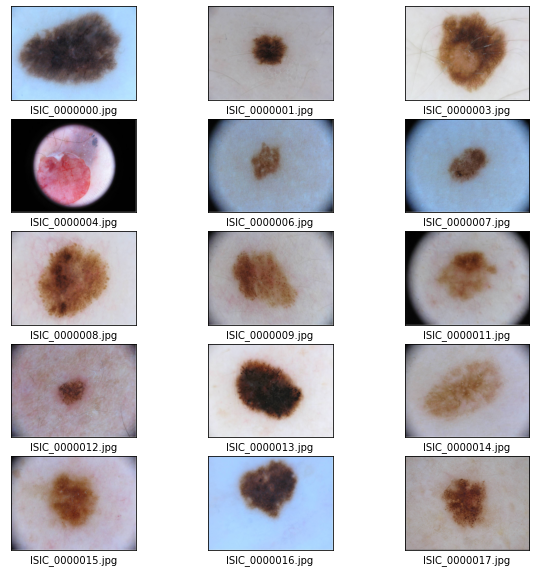
\includegraphics[scale=0.7]{../Plots/Images_input.png}
    \caption{Muestra del conjunto de datos usados para el experimento.}
    \label{fig:img_in}    
\end{figure}

Para este experimento es importante considerar que una intensidad de $\text{pixel} = 0$, en una escala de grises significa que sería completamente negro, mientras que si $\text{pixel} = 255$, significa que el pixel es completamente blanco. Lo mismo aplica a las imágenes a color pero en su correspondiente canal. 

\begin{figure}[]
    \centering
    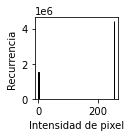
\includegraphics[]{../Plots/threshold_input.png}
    \caption{Histogramas sobre la intensidad de píxeles en el conjunto.}
    \label{fig:hist_in}    
\end{figure}

Los píxeles de las imágenes de entrada tienen una forma de $m \times n$, por lo que para evaluar la intensidad de todos los píxeles es necesario aplanar la dimensión del arreglo, para esto se utilizó la función \texttt{Ravel} de \texttt{NumPy}, la cuál da como resultado un arreglo de una sola dimensión a partir de un arreglo de varias dimensiones o con subarreglos.


\begin{figure}[]
    \centering
    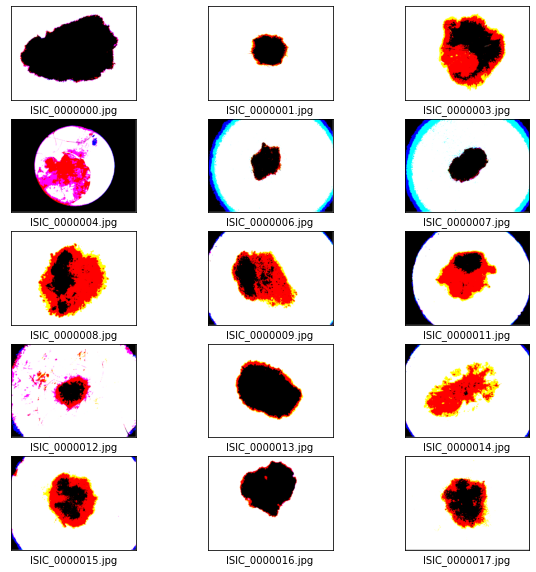
\includegraphics[scale=0.7]{../Plots/Images_output.png}
    \caption{Conjunto de datos después del filtro de umbral.}
    \label{fig:img_out}    
\end{figure}

\begin{figure}[]
    \centering
    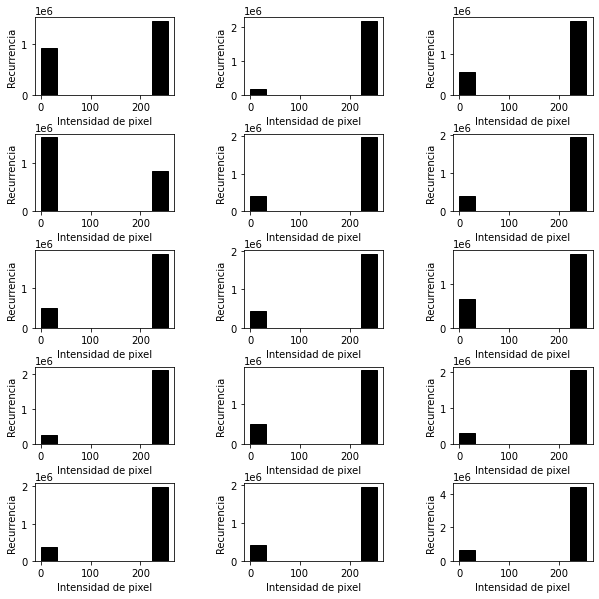
\includegraphics[scale=0.65]{../Plots/threshold_output.png}
    \caption{Histograma de intensidad de píxeles después del filtro de umbral.}
    \label{fig:hist_out}    
\end{figure}

\subsection{Discusión}

\section{Evaluación del Aprendizaje}
Una vez seleccionado el codificador ideal, es necesario evaluar la configuración del modelo en la época presente y configuración actual, al finalizar cada ciclo de entrenamiento se realiza una validación con el porcentaje del conjunto de datos que no fue utilizado durante éste.
\subsection{Diseño Experimental}
Para determinar un valor probabilistico entre dos mapas de valores binarios es necesario utilizar un coeficiente que evalúe la similitud entre ambos conjuntos de datos, siendo el conjunto $A$ la máscara real o \emph{ground truth}, y el conjunto $B$ el mapa obtenido por la computación del modelo se utilizó el criterio de dados para determinar la probabilidad ($0 \% - 100 \%$), la ecuación del criterio de dados dice que la probabilidad de que dos mapas binarios sean iguales es dos veces la cantidad de pixeles sobrepuestos o idénticos entre la suma de los pixeles de ambos mapas, 
\begin{equation}\label{eq:diceloss}
    \text{DC} = \frac{2|A \cap B |}{|A| + |B|}
\end{equation}
donde $A$ es un mapa binario de pixeles que representa la máscara real y $B$ la máscara de segmentación obtenida por el modelo.

\def\firstcircle{(0,0) circle (1.5cm)}
\def\secondcircle{(2,0) circle (1.5cm)}
\def\thirdcircle{(0:2cm) circle (1.5cm)}

\begin{figure}[b]
    \centering
    \begin{tikzpicture}
        \draw \firstcircle node [above] {$A$};
        \draw \secondcircle node [above] {$B$};
        %\node at (-2, 0) {\large $2 \times$};
        \begin{scope}
            \clip \firstcircle;
            \fill[red!20] \secondcircle;
        \end{scope}
    \end{tikzpicture}
    \caption{Representación de la región de sobreposición de pixeles en el coeficiente de dados.}
\end{figure}

\subsection{Resultados}
Durante el entrenamiento del modelo, se evaluó la perdida o el error mediante el coeficiente de dados, dicha evaluación fue realizada en cada iteración y los datos fueron registrados para posteriormente graficar la curva. La curva de la pérdida debe tender a descender cuando el modelo mejora su precisión, al terminar todas las iteraciones se vuelve a pasar el modelo por el proceso de entrenamiento utilizando la configuración del modelo anterior hasta llegar a la mejor precisión posible. En la figura \ref{fig:dice_loss_epochs}, se puede observar la curva en cada una de las épocas.
\begin{figure*}[!b]
    \centering
    \begin{tabular}{ccc}
        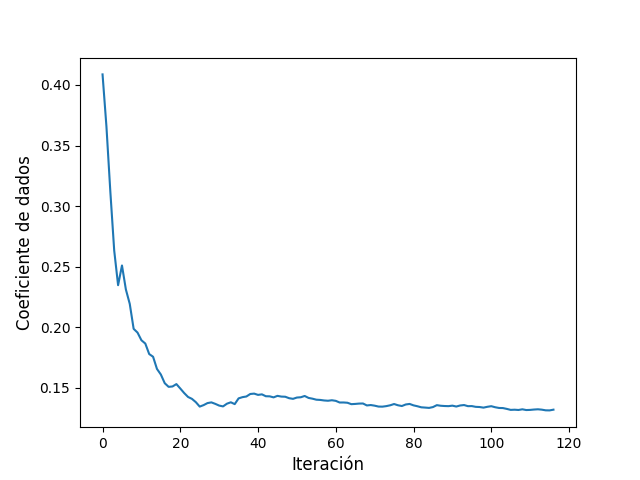
\includegraphics[width=4cm]{../Plots/dl_epoch_0.png} &
        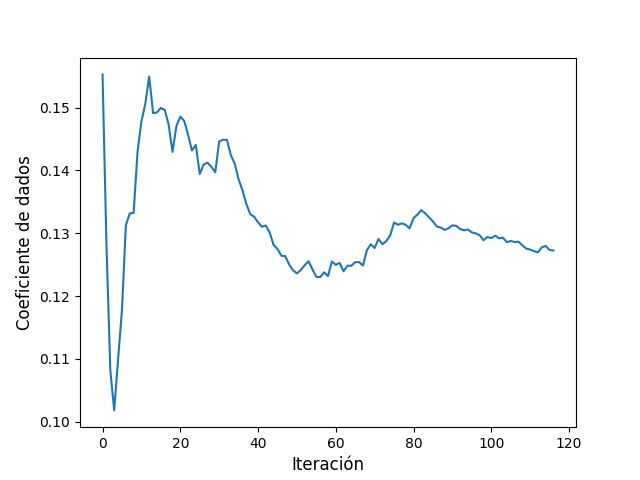
\includegraphics[width=4cm]{../Plots/dl_epoch_1.png} &
        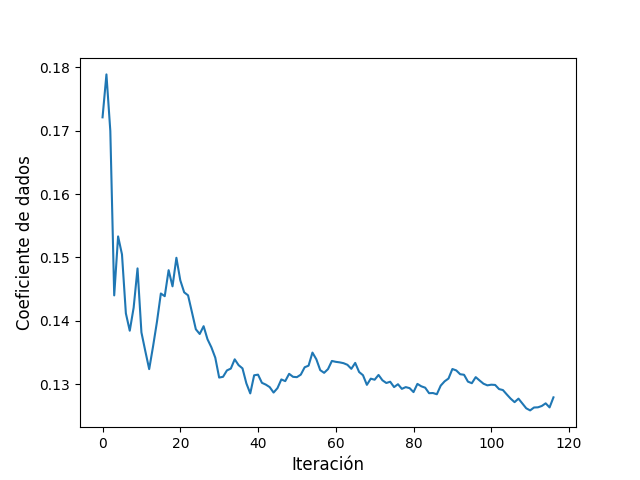
\includegraphics[width=4cm]{../Plots/dl_epoch_2.png} \\

        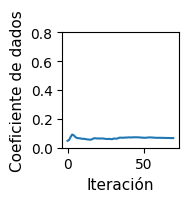
\includegraphics[width=4cm]{../Plots/dl_epoch_3.png} &
        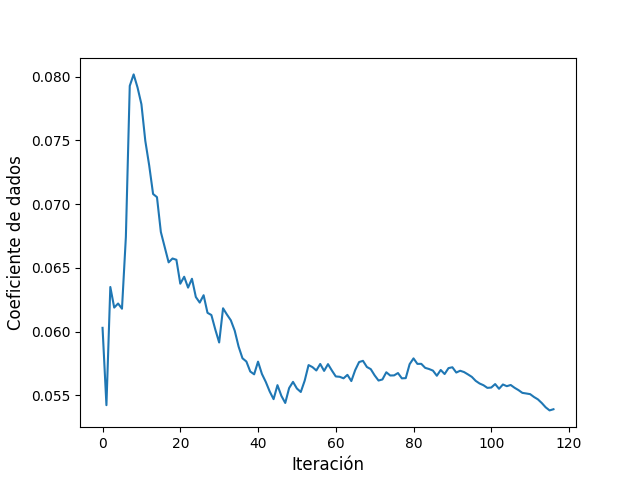
\includegraphics[width=4cm]{../Plots/dl_epoch_4.png} &
        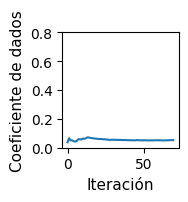
\includegraphics[width=4cm]{../Plots/dl_epoch_5.png} \\

        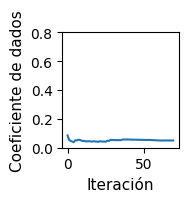
\includegraphics[width=4cm]{../Plots/dl_epoch_6.png} &
        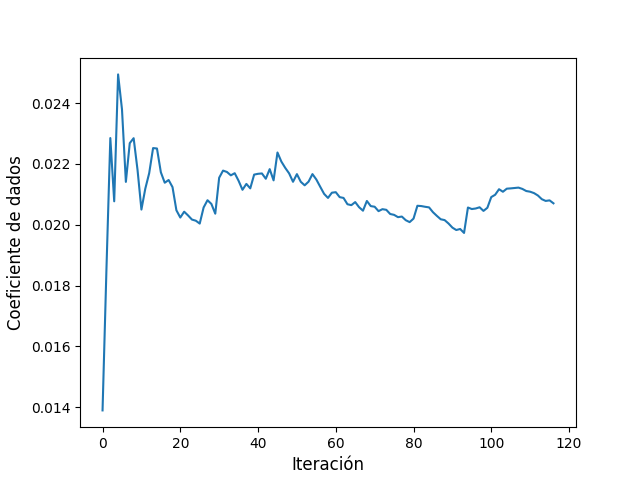
\includegraphics[width=4cm]{../Plots/dl_epoch_7.png} &
        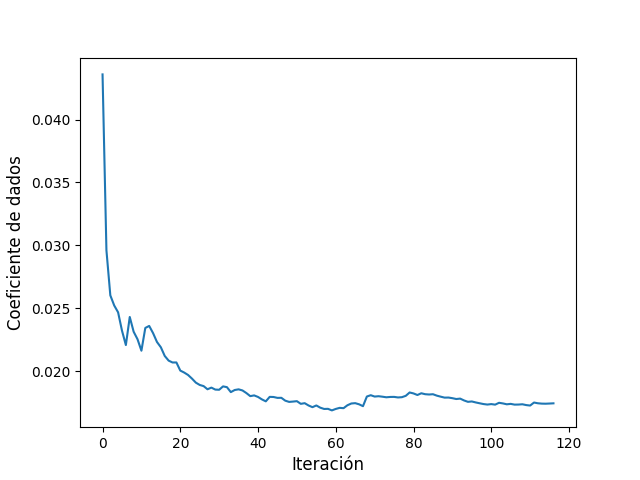
\includegraphics[width=4cm]{../Plots/dl_epoch_8.png} \\

    \end{tabular}        
    \caption{Curva de la pérdida según el coeficiente de dados en cada época.}
    \label{fig:dice_loss_epochs}
\end{figure*}

\begin{figure*}[ht]
    \centering
    \begin{tabular}{ccc}\ContinuedFloat

        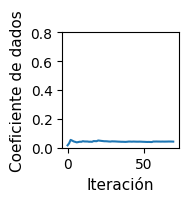
\includegraphics[width=4cm]{../Plots/dl_epoch_9.png} &
        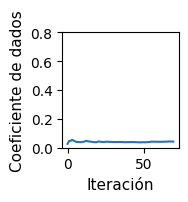
\includegraphics[width=4cm]{../Plots/dl_epoch_10.png} &
        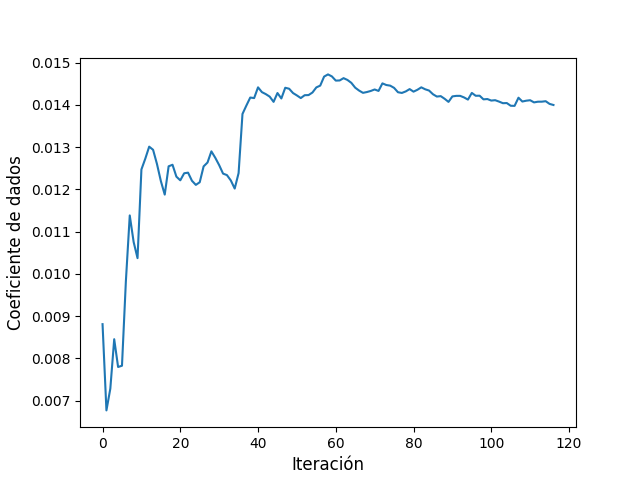
\includegraphics[width=4cm]{../Plots/dl_epoch_11.png} \\

        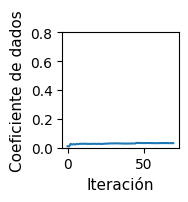
\includegraphics[width=4cm]{../Plots/dl_epoch_12.png} &
        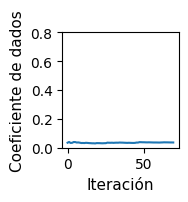
\includegraphics[width=4cm]{../Plots/dl_epoch_13.png} &
        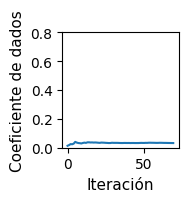
\includegraphics[width=4cm]{../Plots/dl_epoch_14.png} \\

        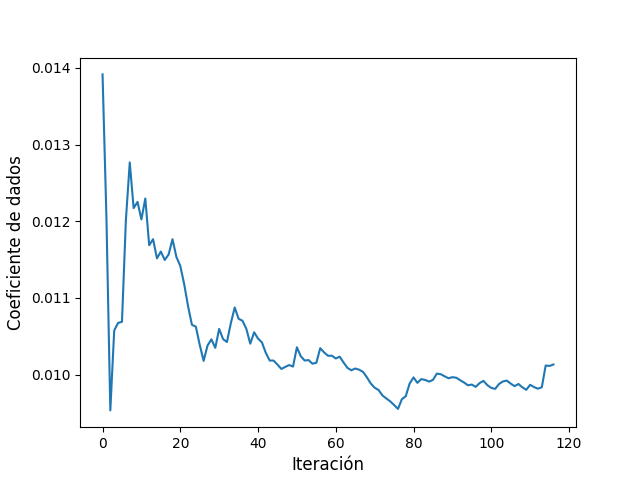
\includegraphics[width=4cm]{../Plots/dl_epoch_15.png} &
        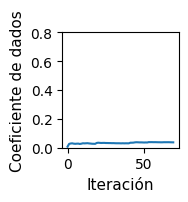
\includegraphics[width=4cm]{../Plots/dl_epoch_16.png} &
        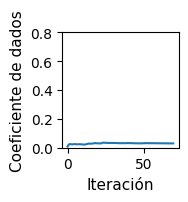
\includegraphics[width=4cm]{../Plots/dl_epoch_17.png} \\
    \end{tabular}        
    \caption{Curva de la pérdida según el coeficiente de dados en cada época.}
    \label{fig:dice_loss_epochs}
\end{figure*}

\subsection{Discusión}
En la sección de resultados muestra en la figura \ref{fig:dice_loss_epochs} la curva de error según el coeficiente de dados, cada gráfica representa una época y sus iteraciones correspondientes. Como se puede observar, en la primera iteración de la primera época el error es mayor, conforme van pasando las épocas la curva se aplana y tiende a cero. Esto nos da a entender que el error disminuye, por lo tanto el modelo se optimiza de forma correcta. 



\section{Criterio de Jaccard}
En la sección anterior, el coeficiente de dados es utilizado para evaluar la diferencia entre un mapa binario y un mapa probabilistico correspondientes a la máscara conocida y la máscara estimada, durante el entrenamiento del modelo. Sin embargo para validar el resultado final es necesario utilizar una métrica muy similar que evalúe ahora la similitud, y que al mismo tiempo penalice más el error.

\subsection{Diseño Experimental}
Para determinar un porcentaje de similitud entre la máscara estimada con la máscara conocida (\emph{ground truth}) podemos utilizar una métrica como la de la ecuación \ref{eq:jacc}, el índice de Jaccard. Este criterio es relativamente similar al coeficiente de dados de la ecuación \ref{eq:diceloss}, mediante el solapado de ambas máscaras se promedía la coincidencia entre pixeles, sin embargo en el criterio de Jaccard \emph{IoU} el error tiene mayor penalización, por lo que se podría decir que es una versión mas estricta de evaluación, lo cual es ideal para evaluar el modelo resultante tras cada época.

La métrica utilizada para evaluar el modelo es la del \emph{índice de Jaccard} (\emph{Intersection Over Union}) por sus siglas en inglés (\emph{IoU}) \citep{fpn_1} de la siguiente ecuación
\begin{equation}\label{eq:jacc}
    J(A,B) = \frac{|A \cap B|}{| A \cup B |} = \frac{|A \cap B|}{|A| + |B| - |A \cap B|} \text{,}
\end{equation} 
donde $A$ y $B$ se pueden interpretar como la máscara real y la máscara estimada, y debido a que las imágenes consisten de pixeles, la ecuación anterior se puede representar también como
\begin{equation}
    J = \frac{1}{n} \sum_{c=1}^{k} W_c \sum_{i=1}^{n}\frac{y_i^c \hat y_i^c}{y_i^c + \hat y_i^c - y_i^c \hat y_i^c} \text{,}
\end{equation} 
donde $y_i^c$ y $\hat y_i^c$ son valores binarios y corresponden a la probabilidad de que el pixel $i$ corresponda a la clase $c$ de un número $k$ de clases.

\def\rectA{(0,0) rectangle (2,2)}
\def\rectB{(1,-1) rectangle (3,1)}

\begin{figure}[h!]
    \centering
    \begin{tikzpicture}
        \draw \rectA node [above] {$A$};
        \draw \rectB node [above] {$B$};
        \begin{scope}
            \clip \rectA;
            \fill[blue!20] \rectB;
        \end{scope}
    \end{tikzpicture}
    \caption{Representación de la región de sobreposición de pixeles en el índice de Jaccard.}
    \label{fig:jacc_inter}
\end{figure}

La figura \ref{fig:jacc_inter} representa, en la forma de un diagrama de Venn, la proporción de píxeles que coinciden (área sombreda) y el error (márgenes), es muy similar a la ecuación del coeficiente de dados sin embargo, tiene una mayor penalización en el error, siendo una mejor métrica post-entrenamiento.

\subsection{Resultados}
Al diferencia de la evaluación mediante el coeficiente de dados,la cual se realiza durante el entrenamiento, la evaluación del criterio de Jaccard se realiza después del entrenamiento, específicamente en la fase de validación donde se vuelve a comparar el mapa de valores binarios real y el mapa probabilístico obtenido con el modelo al finalizar la época presente y dando una mayor penalización al error. En la figura \ref{fig:iou_epochs} se puede observar la forma que la curva toma a través de las iteraciones y su evolución en cada época.

\begin{figure*}[!b]
    \centering
    \begin{tabular}{ccc}
        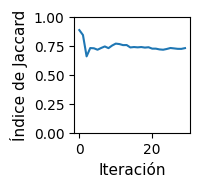
\includegraphics[width=4.5cm]{../Plots/score_epoch_0.png} &
        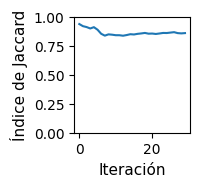
\includegraphics[width=4.5cm]{../Plots/score_epoch_1.png} &
        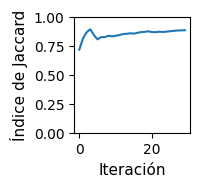
\includegraphics[width=4.5cm]{../Plots/score_epoch_2.png} \\

        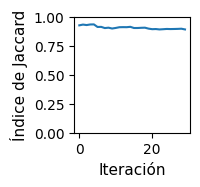
\includegraphics[width=4.5cm]{../Plots/score_epoch_3.png} &
        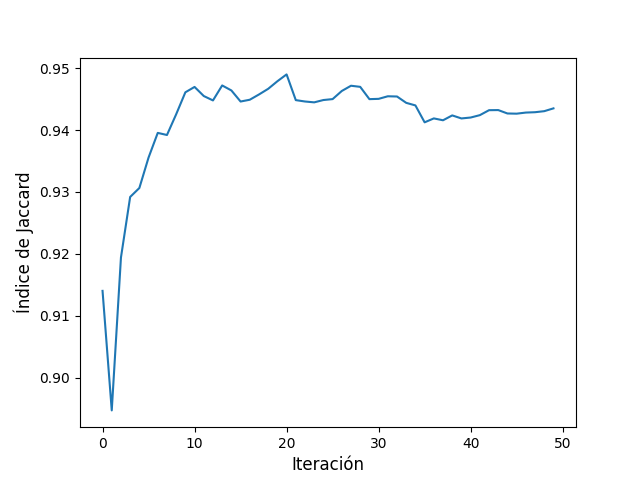
\includegraphics[width=4.5cm]{../Plots/score_epoch_4.png} &
        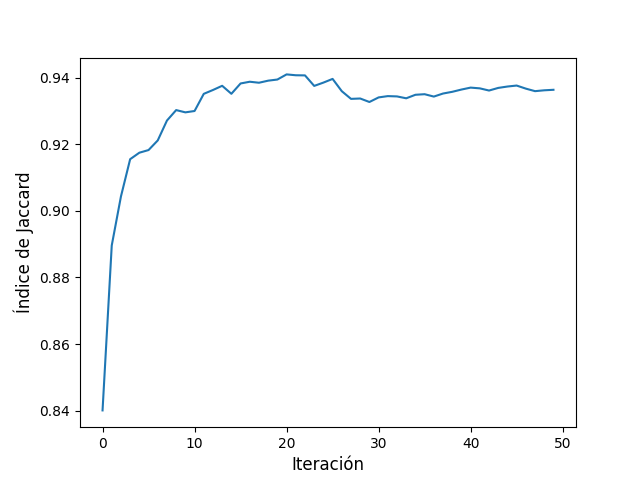
\includegraphics[width=4.5cm]{../Plots/score_epoch_5.png} \\

        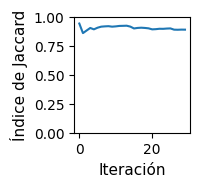
\includegraphics[width=4.5cm]{../Plots/score_epoch_6.png} &
        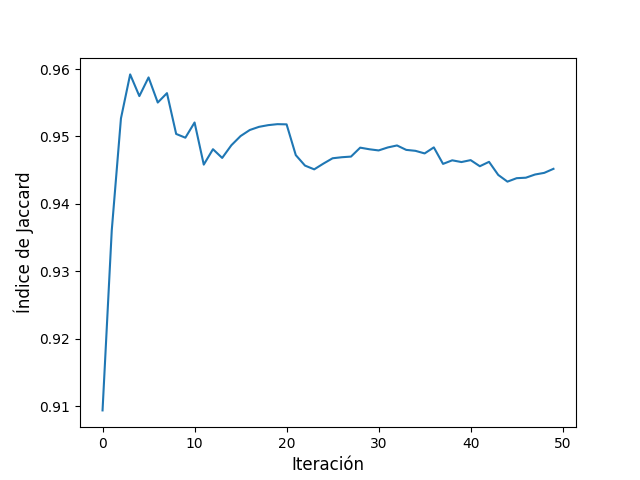
\includegraphics[width=4.5cm]{../Plots/score_epoch_7.png} &
        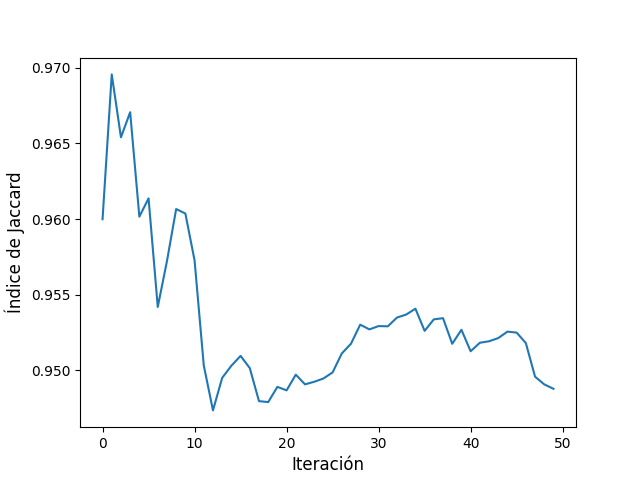
\includegraphics[width=4.5cm]{../Plots/score_epoch_8.png} \\
        
    \end{tabular}
    \caption{Curvas de la evaluación del criterio de Jaccard en cada época.}
    \label{fig:iou_epochs}
\end{figure*}

\begin{figure*}[ht]\ContinuedFloat
    \centering
    \begin{tabular}{ccc}

        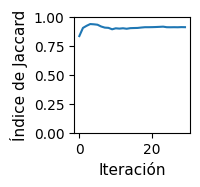
\includegraphics[width=4.5cm]{../Plots/score_epoch_9.png} &
        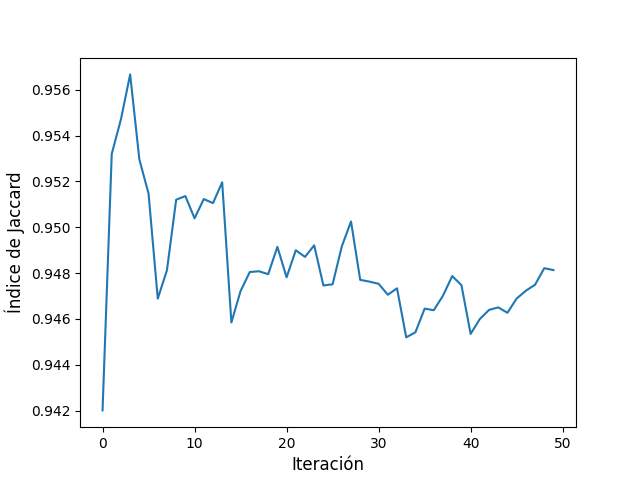
\includegraphics[width=4.5cm]{../Plots/score_epoch_10.png} &
        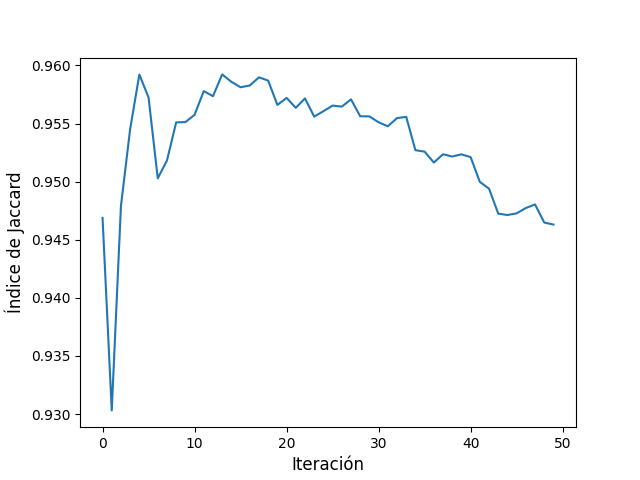
\includegraphics[width=4.5cm]{../Plots/score_epoch_11.png} \\

        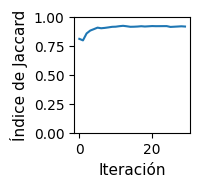
\includegraphics[width=4.5cm]{../Plots/score_epoch_12.png} &
        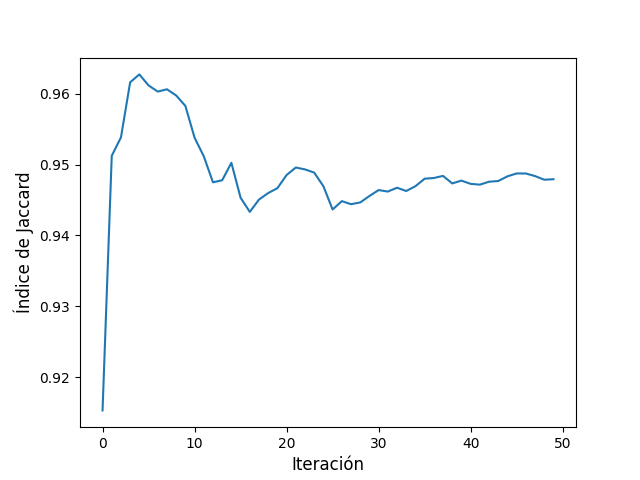
\includegraphics[width=4.5cm]{../Plots/score_epoch_13.png} &
        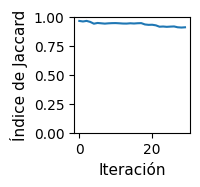
\includegraphics[width=4.5cm]{../Plots/score_epoch_14.png} \\

        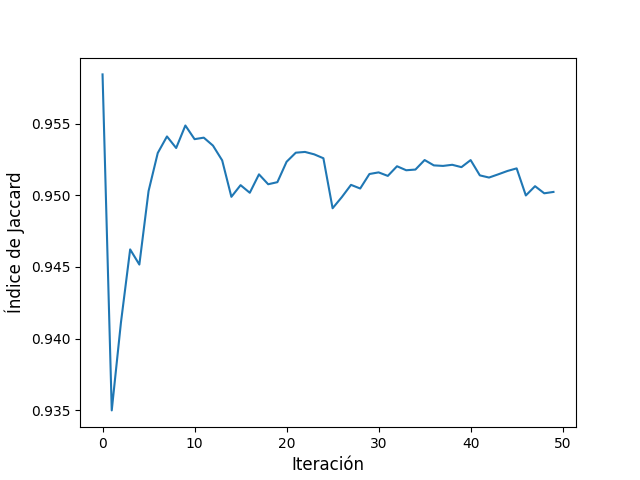
\includegraphics[width=4.5cm]{../Plots/score_epoch_15.png} &
        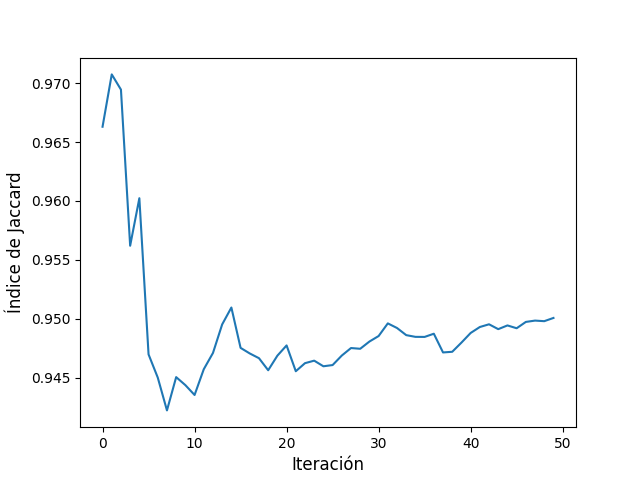
\includegraphics[width=4.5cm]{../Plots/score_epoch_16.png} &
        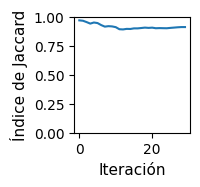
\includegraphics[width=4.5cm]{../Plots/score_epoch_17.png} \\
    \end{tabular}

    \caption{Curvas de la evaluación del criterio de Jaccard en cada época.}
    \label{fig:iou_epochs}
\end{figure*}

\subsection{Discusión}
Una vez finalizado el experimento del criterio de Jaccard, se obtuvieron las gráficas correspondientes a cada época y sus iteraciones. En la figura \ref{fig:iou_epochs} se puede observar en la curva el nivel de similitud, en un principio la precisión del modelo fluctúa al rededor del 75\% y conforme van avanzando las épocas, la curva se endereza y la precisión alcanza un 96\% aproximadamente.

\chapter{Conclusiones}
\section{Discusión}

\section{Trabajo a Futuro}

\nocite{*}

\appendix
%%% Haz un documento para cada apéndice, si es que tienes

\backmatter
\pagestyle{main}

% Aquí va la bibliografía, puedes usar el entorno de LaTeX (thebibliography)
% o la herramienta BibTeX. En caso de que optes por BibTeX, puedes usar
% alguno de los archivos de estilo (mighelbib.bst o mighelnat.bst) incluidos
% en el paquete, cuyos diseños armonizan con el diseño de tesis provisto por
% fime.cls. Para muestra, basta un botón:

\printnoidxglossary[sort=word]

\bibliographystyle{mighelnat}
\bibliography{MiBiblio}
\addcontentsline{toc}{chapter}{Bibliografía}

\label{lastpage}
%Autobiografia

\chapter*{Resumen autobiográfico}
\thispagestyle{empty}

\begin{center}
\autor

Candidato para obtener el grado de\\
\grado\\
\orientacion\bigskip

\uanl\\
\fime\bigskip

Tesis:\\
\textsc{\large\titulo}
\end{center}\bigskip

%Aquí va tu historia
Nací el 4 de junio de 1997 en la ciudad de Monterrey, Nuevo León. Hijo del Sr. Mario Alberto Flores Rosales y la Sra. Patricia Hernández Romero. Comencé mis estudios de Ingeniería en Mecatrónica en agosto de 2014 en la \uanl, en marzo de 2019 llevé a cabo el diplomado de Innovación Biomédica.


\end{document}

